%%%%%%%%%%%%%%%%%%%%%%%%%%%%%%%%%%%%%%%%%
% Masters/Doctoral Thesis 
% LaTeX Template
% Version 2.5 (27/8/17)
%
% This template was downloaded from:
% http://www.LaTeXTemplates.com
%
% Version 2.x major modifications by:
% Vel (vel@latextemplates.com)
%
% This template is based on a template by:
% Steve Gunn (http://users.ecs.soton.ac.uk/srg/softwaretools/document/templates/)
% Sunil Patel (http://www.sunilpatel.co.uk/thesis-template/)
%
% Template license:
% CC BY-NC-SA 3.0 (http://creativecommons.org/licenses/by-nc-sa/3.0/)
%
%%%%%%%%%%%%%%%%%%%%%%%%%%%%%%%%%%%%%%%%%

%----------------------------------------------------------------------------------------
%	PACKAGES AND OTHER DOCUMENT CONFIGURATIONS
%----------------------------------------------------------------------------------------

\documentclass[
11pt, % The default document font size, options: 10pt, 11pt, 12pt
%oneside, % Two side (alternating margins) for binding by default, uncomment to switch to one side
english, % ngerman for German
singlespacing, % Single line spacing, alternatives: onehalfspacing or doublespacing
%draft, % Uncomment to enable draft mode (no pictures, no links, overfull hboxes indicated)
%nolistspacing, % If the document is onehalfspacing or doublespacing, uncomment this to set spacing in lists to single
%liststotoc, % Uncomment to add the list of figures/tables/etc to the table of contents
%toctotoc, % Uncomment to add the main table of contents to the table of contents
%parskip, % Uncomment to add space between paragraphs
%nohyperref, % Uncomment to not load the hyperref package
headsepline, % Uncomment to get a line under the header
%chapterinoneline, % Uncomment to place the chapter title next to the number on one line
%consistentlayout, % Uncomment to change the layout of the declaration, abstract and acknowledgements pages to match the default layout
]{MastersDoctoralThesis} % The class file specifying the document structure
\usepackage{float}
\usepackage{graphicx}
\usepackage{caption}
\usepackage{subcaption}
\usepackage[utf8]{inputenc} % Required for inputting international characters
\usepackage[T1]{fontenc} % Output font encoding for international characters
% \usepackage{etoc}
% \etocsettocstyle{\subsection*{Contents:}}{\noindent\rule{\linewidth}{.4pt}}
\usepackage{titletoc}

\usepackage{mathpazo} % Use the Palatino font by default

\usepackage{amsmath}

\usepackage[backend=biber,style=numeric,natbib=true,maxnames=9]{biblatex} % Use the bibtex backend with the authoryear citation style (which resembles APA)
\addbibresource{references.bib}
\newcommand{\procspie}{Proceedings of the SPIE}
\addbibresource{example.bib} % The filename of the bibliography

\usepackage[autostyle=true]{csquotes} % Required to generate language-dependent quotes in the bibliography

\newcommand\numberthis{\addtocounter{equation}{1}\tag{\theequation}}

\usepackage{listings}
\usepackage{color}
\usepackage{rotating}
\usepackage{tikz}

\definecolor{dkgreen}{rgb}{0,0.6,0}
\definecolor{gray}{rgb}{0.5,0.5,0.5}
\definecolor{mauve}{rgb}{0.58,0,0.82}

\lstset{frame=tb,
  language=Python,
  aboveskip=3mm,
  belowskip=3mm,
  showstringspaces=false,
  columns=flexible,
  basicstyle={\small\ttfamily},
  numbers=none,
  numberstyle=\tiny\color{gray},
  keywordstyle=\color{blue},
  commentstyle=\color{dkgreen},
  stringstyle=\color{mauve},
  breaklines=true,
  breakatwhitespace=true,
  tabsize=3
}

%----------------------------------------------------------------------------------------
%	MARGIN SETTINGS
%----------------------------------------------------------------------------------------

\geometry{
	paper=a4paper, % Change to letterpaper for US letter
	inner=2.5cm, % Inner margin
	outer=3.8cm, % Outer margin
	bindingoffset=.5cm, % Binding offset
	top=1.5cm, % Top margin
	bottom=1.5cm, % Bottom margin
	%showframe, % Uncomment to show how the type block is set on the page
}

%----------------------------------------------------------------------------------------
%	THESIS INFORMATION
%----------------------------------------------------------------------------------------

\thesistitle{Design and Demonstration of Focal Plane Wavefront sensing for co-phasing the GMT} % Your thesis title, this is used in the title and abstract, print it elsewhere with \ttitle
\supervisor{Dr. Kelsey Miller \\ \& Prof. Matthew Kenworthy \\ \& MSc. Steven Bos} % Your supervisor's name, this is used in the title page, print it elsewhere with \supname

\examiner{Prof. Matthew Kenworthy} % Your examiner's name, this is not currently used anywhere in the template, print it elsewhere with \examname
\degree{Masters Thesis} % Your degree name, this is used in the title page and abstract, print it elsewhere with \degreename
\author{Alex Tripsas} % Your name, this is used in the title page and abstract, print it elsewhere with \authorname
\addresses{} % Your address, this is not currently used anywhere in the template, print it elsewhere with \addressname

\subject{Astronomy and Instrumentation} % Your subject area, this is not currently used anywhere in the template, print it elsewhere with \subjectname
\keywords{AO, SLAO, WFS, ZEMAX, Adaptive, Optics} % Keywords for your thesis, this is not currently used anywhere in the template, print it elsewhere with \keywordnames
\university{Leiden University} % Your university's name and URL, this is used in the title page and abstract, print it elsewhere with \univname
\department{Astronomy and Instrumentation} % Your department's name and URL, this is used in the title page and abstract, print it elsewhere with \deptname
% \group{} % Your research group's name and URL, this is used in the title page, print it elsewhere with \groupname
\faculty{Astronomy Department} % Your faculty's name and URL, this is used in the title page and abstract, print it elsewhere with \facname

\AtBeginDocument{
\hypersetup{pdftitle=\ttitle} % Set the PDF's title to your title
\hypersetup{pdfauthor=\authorname} % Set the PDF's author to your name
\hypersetup{pdfkeywords=\keywordnames} % Set the PDF's keywords to your keywords
}

\begin{document}

\frontmatter % Use roman page numbering style (i, ii, iii, iv...) for the pre-content pages

\pagestyle{plain} % Default to the plain heading style until the thesis style is called for the body content

%----------------------------------------------------------------------------------------
%	TITLE PAGE
%----------------------------------------------------------------------------------------

\begin{titlepage}
\begin{center}

\vspace*{.06\textheight}
{\scshape\LARGE \univname\par}\vspace{1.5cm} % University name
\textsc{\Large Masters Thesis}\\[0.5cm] % Thesis type

\HRule \\[0.4cm] % Horizontal line
{\huge \bfseries \ttitle\par}\vspace{0.4cm} % Thesis title
\HRule \\[1.5cm] % Horizontal line
 
\begin{minipage}[t]{0.4\textwidth}

\begin{flushleft} \large
\emph{Author:}\\
\href{http://www.johnsmith.com}{\authorname} % Author name - remove the \href bracket to remove the link
\end{flushleft}
\end{minipage}
\begin{minipage}[t]{0.4\textwidth}
\begin{flushright} \large
\emph{Supervisor:} \\
\href{http://www.jamessmith.com}{\supname} % Supervisor name - remove the \href bracket to remove the link  
\end{flushright}
\end{minipage}\\[3cm]
 
\vfill

\large \textit{A thesis submitted in fulfillment of the requirements\\ for the degree of \degreename}\\[0.3cm] % University requirement text
\textit{in the department for}\\[0.4cm]
\deptname\\[2cm] % Research group name and department name
 
\vfill

{\large \today}\\[4cm] % Date
%\includegraphics{Logo} % University/department logo - uncomment to place it
 
\vfill
\end{center}
\end{titlepage}

%----------------------------------------------------------------------------------------
%	DECLARATION PAGE
%----------------------------------------------------------------------------------------

\begin{declaration}
\addchaptertocentry{\authorshipname} % Add the declaration to the table of contents
\noindent I, \authorname, declare that this thesis titled, \enquote{\ttitle} and the work presented in it are my own. I confirm that:

\begin{itemize} 
\item This work was done wholly or mainly while in candidature for a research degree at this University.
\item Where any part of this thesis has previously been submitted for a degree or any other qualification at this University or any other institution, this has been clearly stated.
\item Where I have consulted the published work of others, this is always clearly attributed.
\item Where I have quoted from the work of others, the source is always given. With the exception of such quotations, this thesis is entirely my own work.
\item I have acknowledged all main sources of help.
\item Where the thesis is based on work done by myself jointly with others, I have made clear exactly what was done by others and what I have contributed myself.
\end{itemize}
 
\noindent Signed:\\
\rule[0.5em]{25em}{0.5pt} % This prints a line for the signature
 
\noindent Date:\\
\rule[0.5em]{25em}{0.5pt} % This prints a line to write the date
\end{declaration}

\cleardoublepage

%----------------------------------------------------------------------------------------
%	QUOTATION PAGE
%----------------------------------------------------------------------------------------

\vspace*{0.2\textheight}

\noindent\enquote{\itshape Now is the moment that everything can change\\
You are completely responsible for your own life\\
And no one is coming to save you from yourself\\
So stop blaming your problems on any or everything else\\
It does not matter one tiny fucking bit\\
How unfair you think the world is\\
It's only what you do\\
Right here, right now\\
Right this fucking instant that matters\\
It's your choice to\\
Sink or swim}\bigbreak

\hfill D. Randall Blythe

%----------------------------------------------------------------------------------------
%	ABSTRACT PAGE
%----------------------------------------------------------------------------------------

\begin{abstract}
\addchaptertocentry{\abstractname} % Add the abstract to the table of contents.
The 25 meter, Giant Magellan Telescope (GMT) will be comprised of seven 8.4 meter mirrors that will have a resolving power ten times greater than that of the Hubble Space Telescope. The GMT will be capable of directly imaging nearby exoplanets with an angular resolution of 10-30 milliarcseconds in the near-IR. To make this possible, the seven separate mirrors need to be co-phased to a fraction of a wavelength to act as one 25 meter aperture. To co-phase the mirrors, we propose to use an Asymmetric Pupil vector Apodizing Phase Plate (APvAPP). The APvAPP generates two science images which can be used to sense aberrations in the pupil.  This focal-plane wavefront sensing (FPWFS) technique will allow for the determination of segment piston, tip, and tilt. For simulation work, the python software package HCIPy was used to optimize the asymmetry of the APvAPP. Simulations are veried in the laboratory with a low-order deformable mirror (DM) to induce and then correct wavefront errors into a liquid crystal APvAPP located in a conjugate pupil plane. Here we present results of the development, optimization, and testing of the APvAPP in the laboratory.
\end{abstract}

%----------------------------------------------------------------------------------------
%	ACKNOWLEDGEMENTS
%----------------------------------------------------------------------------------------

\begin{acknowledgements}
\addchaptertocentry{\acknowledgementname} % Add the acknowledgements to the table of contents

I'd like to thank Dr. Kelsey Miller 

Steven Bos 

To all my old colleagues back at University of California Santa Cruz for, despite me not being there anymore, to continue to help me.  Notably, Will Deich, if it weren't for you, this research would have been a nightmare.  

Lastly, Professor Matthew Kenworthy


\end{acknowledgements}

%----------------------------------------------------------------------------------------
%	LIST OF CONTENTS/FIGURES/TABLES PAGES
%----------------------------------------------------------------------------------------

\tableofcontents % Prints the main table of contents

\listoffigures % Prints the list of figures

\listoftables % Prints the list of tables

%----------------------------------------------------------------------------------------
%	ABBREVIATIONS
%----------------------------------------------------------------------------------------

\begin{abbreviations}{ll} % Include a list of abbreviations (a table of two columns)

  \textbf{GMT} & Giant Magellan Telescope\\
  \textbf{PSF} & Point Spread Function\\
  \textbf{DM} & Deformable Mirror \\
  \textbf{AO} & Adaptive Optics \\
  \textbf{WFS} & WaveFront Sensor \\
  \textbf{FPWFS} & Focal Plane Wavefront Sensing \\
  



\end{abbreviations}

%----------------------------------------------------------------------------------------
%	PHYSICAL CONSTANTS/OTHER DEFINITIONS
%----------------------------------------------------------------------------------------

% \begin{constants}{lr@{${}={}$}l} % The list of physical constants is a three column table

% % The \SI{}{} command is provided by the siunitx package, see its documentation for instructions on how to use it

% Speed of Light & $c_{0}$ & \SI{2.99792458e8}{\meter\per\second} (exact)\\
% %Constant Name & $Symbol$ & $Constant Value$ with units\\

% \end{constants}

%----------------------------------------------------------------------------------------
%	SYMBOLS
%----------------------------------------------------------------------------------------

% \begin{symbols}{lll} % Include a list of Symbols (a three column table)

% $a$ & distance & \si{\meter} \\
% $P$ & power & \si{\watt} (\si{\joule\per\second}) \\
% %Symbol & Name & Unit \\

% \addlinespace % Gap to separate the Roman symbols from the Greek

% $\omega$ & angular frequency & \si{\radian} \\

% \end{symbols}

%----------------------------------------------------------------------------------------
%	DEDICATION
%----------------------------------------------------------------------------------------

\dedicatory{Dedicated to my friends and family who helped keep me going.} 

%----------------------------------------------------------------------------------------
%	THESIS CONTENT - CHAPTERS
%----------------------------------------------------------------------------------------

\mainmatter % Begin numeric (1,2,3...) page numbering

\pagestyle{thesis} % Return the page headers back to the "thesis" style

% Include the chapters of the thesis as separate files from the Chapters folder
% Uncomment the lines as you write the chapters
% \dominitoc

% Chapter Template

\chapter{Introduction} % Main chapter title

\noindent\textbf{\large Contents:}

\noindent\hrulefill
\noindent\startcontents[chapters]
\noindent\printcontents[chapters]{}{1}{}
\noindent\hrulefill

\label{Chapter1} % Change X to a consecutive number; for referencing this chapter elsewhere, use \ref{ChapterX}

Advances in astronomy come in many forms, from the exploration of new theories to new observational techniques.
But astronomy would not be possible without the main tool of the astronomer, the telescope.  Starting from when
Galileo Galilei first pointed his telescope to the night sky, astronomers have been demanding more from their
telescopes.  The only way to enhance a telescopes resolving power is to increase the primary aperture of the
telescope.  In the early 1900's telescopes were made up of a large single optics for the primary aperture. 
However, there is a limit to how large you can make a single optic.  

Eventually, these mirrors were becoming so
large that the mirrors would sag under their own weight.  These large optics quickly became heavier and needed
more mechanical supports.  In order to solve this problem, a honeycomb substructure was designed to keep the
mirrors lighter and more ridged.  Figure \ref{fig:hale} shows the primary mirror of the 200-inch Hale telescope
and backlight to show the structure.  While this helped keep large single optics rigid, there is still a limit
to how large one optic can be.  The University of Arizona's Large Optics Facility is capable of constructing
8.4 meter mirrors \cite{LOFTSystems.}.  One of the reasons for this limit is that this is roughly the maximum
width of bridge underpasses in Arizona.  In order to achieve larger primary apertures, a different approach is
needed.


\begin{figure}[!h]
\centering
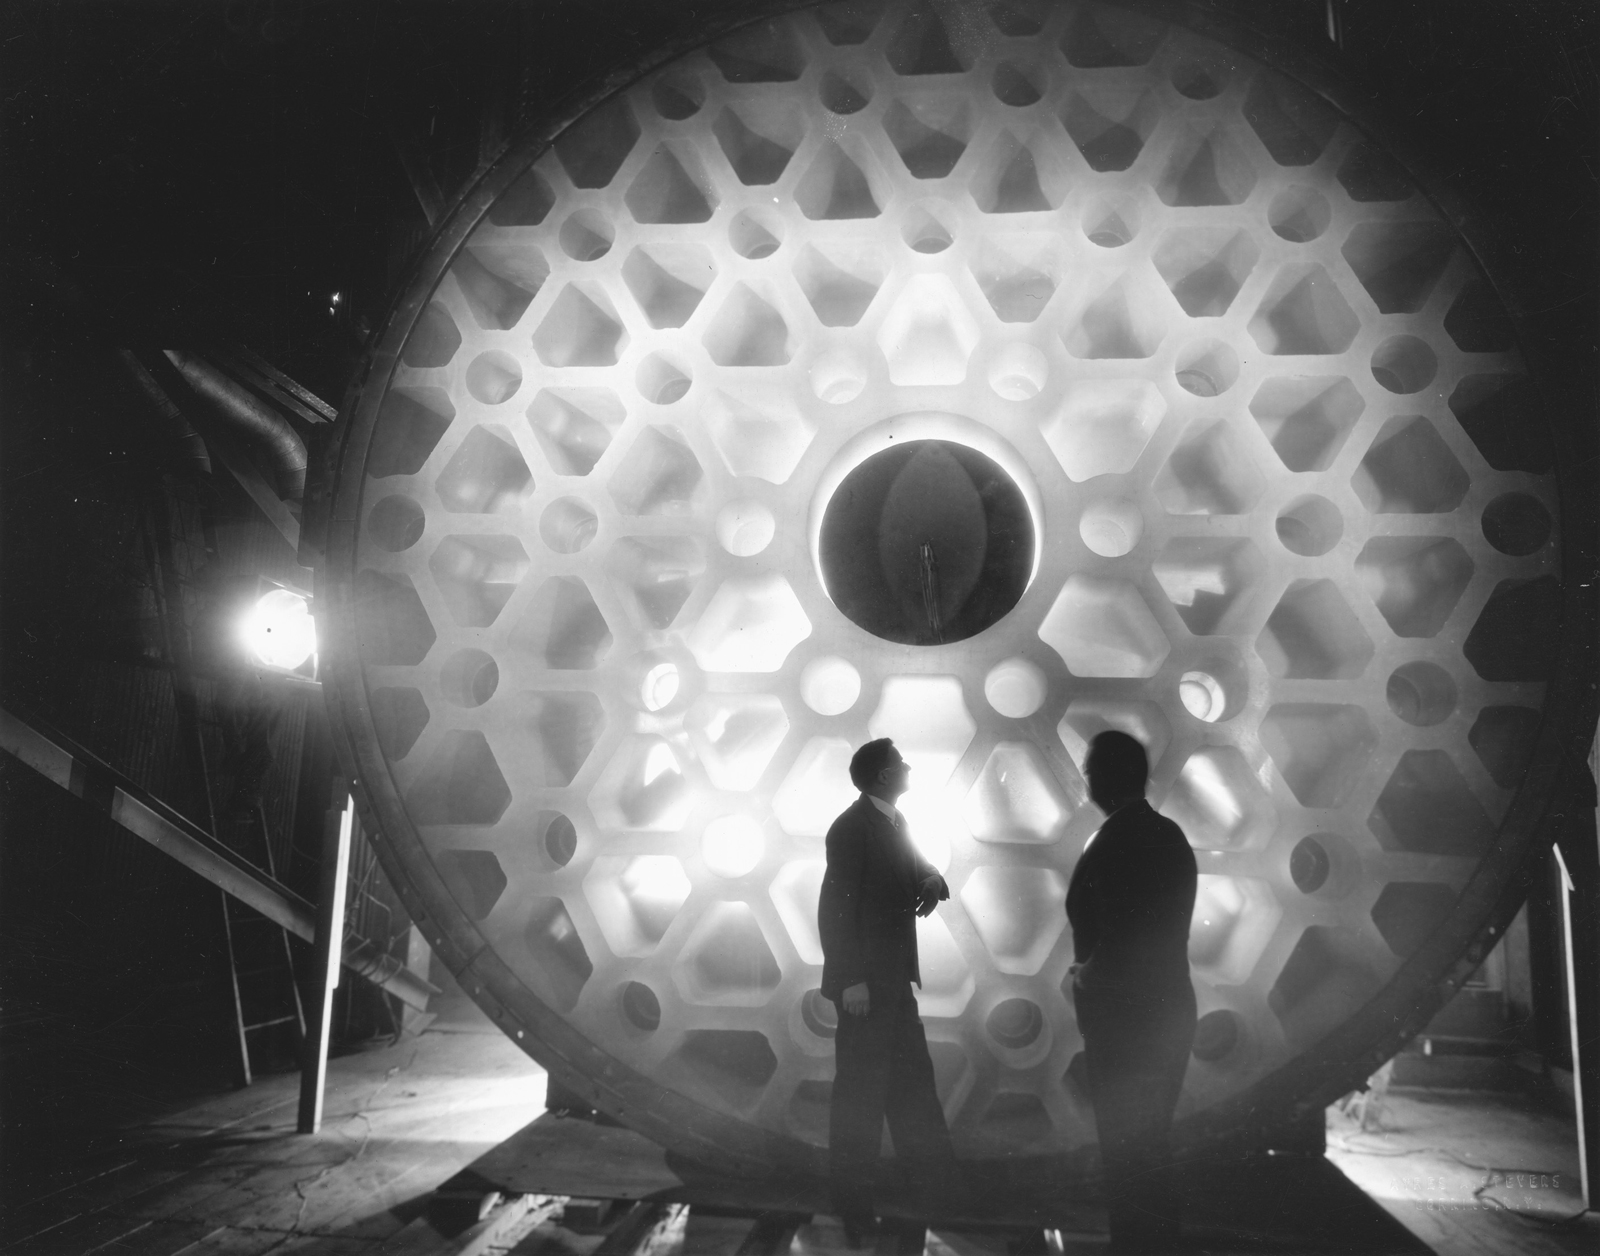
\includegraphics[width=12 cm]{../Figures/twomen}
\caption{Image of the Hale 200-inch (5.1m) primary mirror.  The honeycomb structure was to reduce the mass of the optic and make the surface more ridged}
\label{fig:hale}
\end{figure}


\section{Segmented Mirrors / Active Optics}
In 1977, Dr. Jerry Nelson and a team of scientists at the Lawrence Berkeley National Laboratory, were tasked with designing a 10-meter telescope \cite{BeatingObservatory}.  



\section{FPWFS}



\section{Vector Apodizing Phase Plate}






\begin{itemize}
    \item Segmented Mirrors
    \item FPWFS
    \item vAPP
    % \item hcipy
\end{itemize}



%----------------------------------------------------------------------------------------
%	SECTION 1
%----------------------------------------------------------------------------------------

% Chapter Template

\chapter{Simulation} % Main chapter title

\noindent\textbf{\large Contents:}

\noindent\hrulefill
\noindent\startcontents[chapters]
\noindent\printcontents[chapters]{}{1}{}
\noindent\hrulefill

\label{Chapter2}% Change X to a consecutive number; for referencing this chapter elsewhere, use \ref{ChapterX}

The simulation portion of this research was to find what the response in the focal plane of our science image would
be if one or more of the segments was out of phase from the rest.  In order to do this, one segment will be isolated
at a time and each of the three modes will be applied to it (Piston, Tip, or Tilt).  All 21 combinations for
P/T/T for all seven segments will be put into a matrix called the response matrix (RM).  All coding was done in
python using the python package HCIpy made in house at Leiden University \cite{por2018hcipy}.  %Further explain HCIpy
HCIpy is a Python framework used for high contrast imaging simulation that is able to implement adaptive optic simulation, coronagraphy and optical diffraction calculations \cite{por2018hcipy}.
This section will go into the process of building the response matrix as well as preparing the FPWFS.


\section{Response Matrix}
\label{sec:RM}

%Using an empirical, linear wavefront estimator (which a RM is).  Also discuss what the advantages and disadvantages are.


Simulations started off with supplied GMT pupil images. %Reword
One was
a binary amplitude mask of the GMT pupil (Figure \ref{fig:amp_mask} and the other was the phase (Figure
\ref{fig:phase_mask}) that would be induced by the vAPP.  Both masks have the asymmetry discussed in \S
\ref{sec:vAPP} in order to detect all of the modal basis set in the focal plane.  

\begin{figure}[H]
\centering
\begin{subfigure}{.5\textwidth}
  \centering
  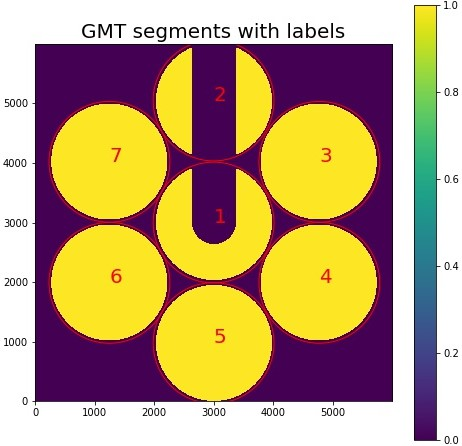
\includegraphics[width=6cm]{Figures/GMT_seg_choice.jpg}
  \caption{Amplitude mask of the GMT pupil.  Each segment is labeled 1-7 for which segment is to be isolated by the code.}
  \label{fig:amp_mask}
\end{subfigure}%
\begin{subfigure}{.5\textwidth}
  \centering
  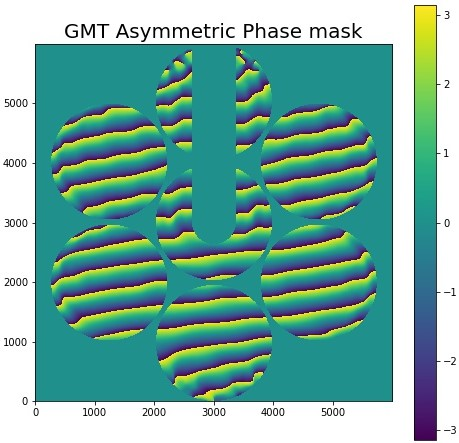
\includegraphics[width=6cm]{Figures/gmt_phase_mask.jpg}
  \caption{GMT phase mask that will be induced by the vAPP.  Each segment has a sinusoidal wave going across each segment.}
  \label{fig:phase_mask}
\end{subfigure}
% \caption{Asymmetric pupil planes used for simulation of the GMT FPWFS test}
\label{fig:asym_pupils}
\end{figure}

%Add image of the nominal PSF

\begin{figure}[H]
\centering
\begin{subfigure}{.5\textwidth}
  \centering
  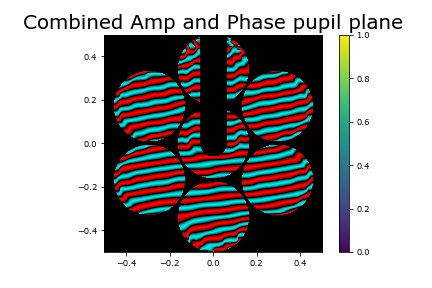
\includegraphics[width=8cm]{Figures/GMT_amp_phase_comb.jpg}
  \caption{The pupil plane after combining the amplitude and phase masks.}
  \label{fig:pupil_comb}
\end{subfigure}%
\begin{subfigure}{.5\textwidth}
  \centering
  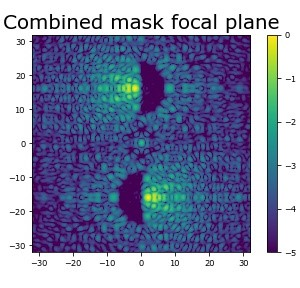
\includegraphics[width=6cm]{Figures/GMT_focal_plane.jpg}
  \caption{Focal plane image of the vAPP PSFs with no modes applied.}
  \label{fig:focal_comb}
\end{subfigure}
% \caption{Asymmetric pupil planes used for simulation of the GMT FPWFS test}
\label{fig:zero_GMT}
\end{figure}


In order to apply aberrations to a segment, individual segments needed to be isolated.  The code makes a circle of
ones roughly the shape of the segment, and zeros across the rest of the array. When the circle mask was multiplied
by Figure \ref{fig:amp_mask} we get the segment isolated (Figure \ref{fig:single_seg}).  With the segment isolated,
we now want to add an aberration to this segment.  As an example I will look at tilt.  With the segment isolated,
the code generates a tip across the entire image and then makes sure that the values range from -1 to 1 only for the
segment (Figure \ref{fig:tilt_seg}).  

\begin{figure}[H]
\centering
\begin{subfigure}{.5\textwidth}
  \centering
  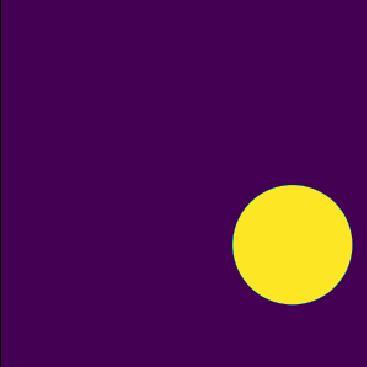
\includegraphics[width=6.5cm]{Figures/isolated_seg.png}
  \caption{Segment 4 isolated by the code.}
  \label{fig:single_seg}
\end{subfigure}%
\begin{subfigure}{.5\textwidth}
  \centering
  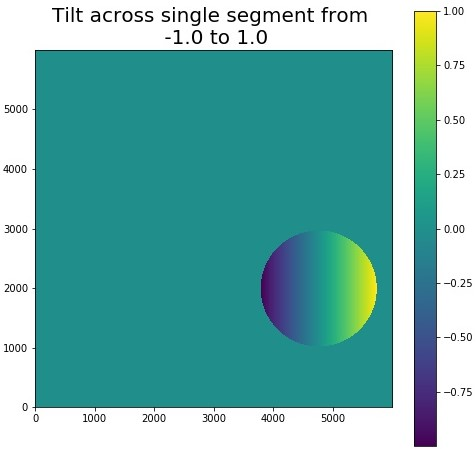
\includegraphics[width=6.5cm]{Figures/tip_single_seg.jpg}
  \caption{Isolated segment with a tilt applied to it.}
  \label{fig:tilt_seg}
\end{subfigure}
\caption{Isolated segment manipulation.  Axes are in pixel units.  Colorbar is for modal amplitudes.}
\label{fig:isolated_seg}
\end{figure}

However, in order to properly simulate phase errors, we need to translate physical values to phase values.
In order
to do this, we will apply an optical path difference (OPD) between the unaberrated segment and the segment with
aberration.  The phase difference is given by:

\begin{equation}
    \phi = 2 \pi \times \frac{d}{\lambda}
    \label{eq:OPD}
\end{equation}

Where $d$ is the amplitude in nanometers of the mode and $\lambda$ is the operation wavelength in the same units.  In this case, $\lambda = 532$nm. 
This is because the vAPP used on our optical testbed was tuned for lasers operating at 532nm.  For simplicity, the
code constructed the matrix for an OPD of 1nm so Equation \ref{eq:OPD} is simplified to $\phi = 2 \pi / \lambda$. 
With the phase difference calculated, it is multiplied by the tilt array (Figure \ref{fig:tilt_seg}), to give us a
segment with the appropriate values.  With the modification done to the segment, next step is to recombine the
aberration (Figure \ref{fig:tilt_seg}), amplitude mask (Figure \ref{fig:amp_mask}, as well as the phase mask (Figure
\ref{fig:phase_mask}).  To do this, I used the following equation:

\begin{equation}
    E = A \times e^{i \phi} \;\;\; \rightarrow \;\;\; I = |E|^2
    \label{eq:intensity}
\end{equation}

Where $I$ is intensity, $A$ is the amplitude (Figure \ref{fig:amp_mask}) and $\phi$ is the phase of light (Figure
\ref{fig:phase_mask}).  However, just using Equation \ref{eq:intensity} will give a unaberrated image.  Using the
phase, we combine the aberration and unaberrated pupil plane in the exponential because these are phase differences. 
This is done for each of the three PSFs that come from the vAPP.  So we now have three different intensity
equations:

\begin{align}
    & E_{top} = A \times e^{(i \cdot (\phi_{ab} + \phi))} \label{eq:top_PSF} \\
    & E_{leakage} = A \times 0.1 \times e^{i \phi_{ab}} \label{eq:leak_PSF} \\
    & E_{bottom} = A \times e^{(-i \phi) + (i \phi_{ab})} \label{eq:bottom_PSF}
\end{align}

Here $\phi_{ab}$ is the phase aberration we previously made, and the multiplication factor of 0.1 for Equation
\ref{eq:leak_PSF} is an intensity approximation of the leakage term.  With all of these combined we get a pupil
plane as shown in Figure \ref{fig:tilt_pupil}.  However, we want to propagate each electric field separately and then add up
the intensities after propagation.  Propagation is done with an inbuilt function of HCIpy called FraunhoferPropagator that assumes that the lens is a perfect propagator \cite{por2018hcipy}.  
After each field is propagated and added together in the focal plane, we get an image like that
in Figure \ref{fig:tilt_focal}.

\begin{figure}[H]
\centering
\begin{subfigure}{.5\textwidth}
  \centering
  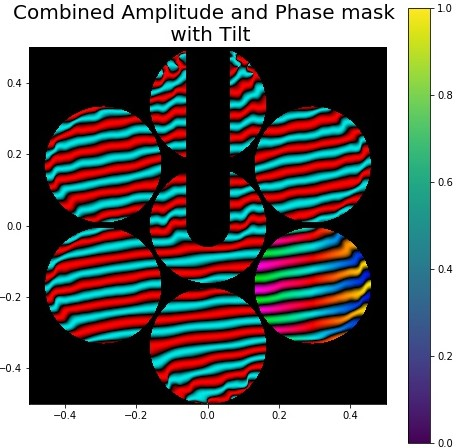
\includegraphics[width=6.5cm]{Figures/tilt_comb.jpg}
  \caption{Pupil image with induced tilt aberration on the lower right hand segments.  Note the change in color compared to Figure \ref{fig:pupil_comb}.}
  \label{fig:tilt_pupil}
\end{subfigure}%
\begin{subfigure}{.5\textwidth}
  \centering
  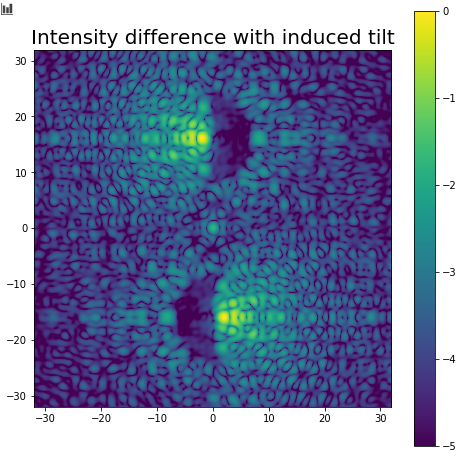
\includegraphics[width=6.5cm]{Figures/PSF_tilt.png}
  \caption{Log scale of focal plane with tilt aberration.}
  \label{fig:tilt_focal}
\end{subfigure}
\caption{Pupil and Focal plane of tilt applied to segment 4.  There is additional intensity in the dark holes compared to Figure \ref{fig:focal_comb}.}
\label{fig:abb_images}
\end{figure}

Last step is to find the negative response in the focal plane for this aberration.  This is simply done by repeating this
process but instead changing Equation \ref{eq:OPD} to have a negative OPD applied to it.  So the equation now
becomes $\phi = -2 \pi / \lambda$.  After repeating the process, we get a new focal plane image.  Now the response
for a tilt on segment 4 can be calculated by taking $I_{pos} - I_{neg}$ (Figure \ref{fig:I_diff}).  This image is
stored as a 1-D vector and all 21 combinations of P/T/T for each of the seven segments are stored in a matrix.  This
is our Response Matrix (RM).  Now that there is a RM, we want to create the inverse of this matrix so that an inputted
aberration can output an amplitude of each mode in our modal basis set (P/T/T).  For a full array of response matrix images please refer to Appendix \ref{AppendixA}.


\begin{figure}[H]
    \centering
    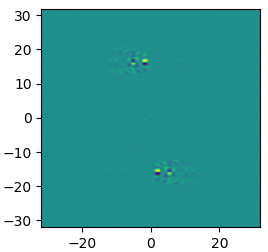
\includegraphics[width = 6cm]{Figures/I_diff.png}
    \caption{Focal plane response for tilt on segment 4.}
    \label{fig:I_diff}
\end{figure}



\section{Control Matrix}
\label{sec:CM}

Construction of the control matrix involves taking a pseudo-inverse of the RM.  This is done using singular value
decomposition of the RM.  Singular value decomposition (SVD) in linear algebra, is a way of decomposing a real or
complex square matrix into the pseudoinverse of a matrix and allows for furhter data analysis to be done \cite{Hestenes1958InversionResults}.  First we decompose
our response matrix $M$ into $M = U \Sigma V^{\ast}$ and the pseudoinverse is:

\begin{equation}
    M^{\dagger} = V \Sigma^{\dagger} U^{\ast}
    \label{eq:SVD}
\end{equation}

\begin{figure}[H]
    \centering
    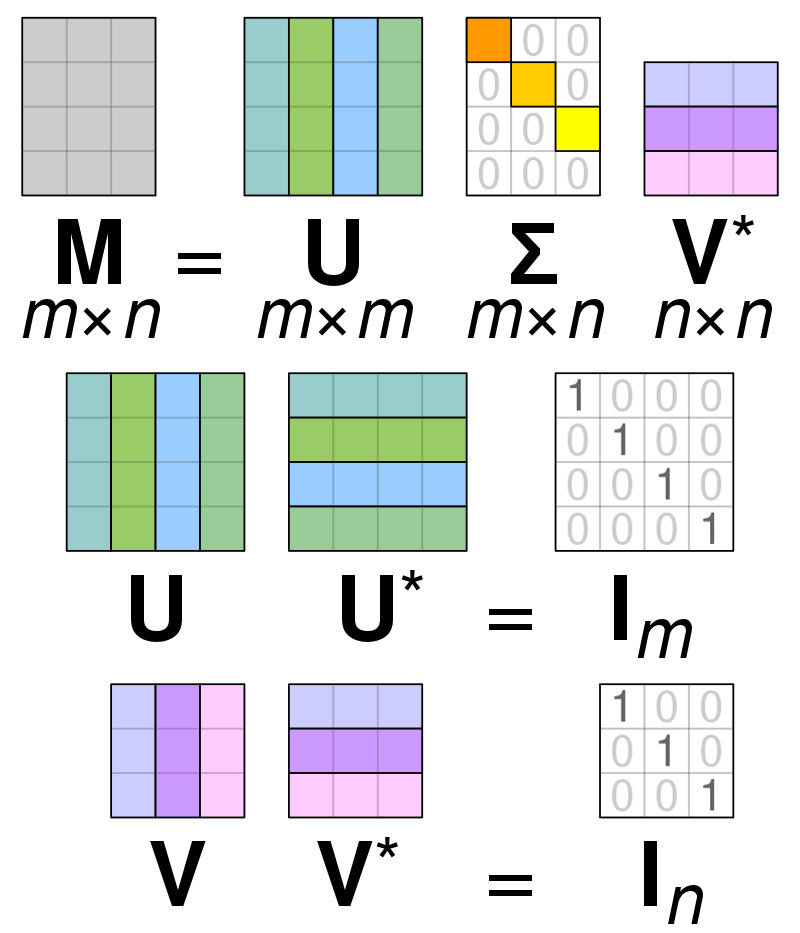
\includegraphics[width = 6cm]{Figures/Singular_value_decomposition_visualisation.jpg}
    \caption{A visual of Singular Value Decomposition \cite{Hestenes1958InversionResults}.}
    \label{fig:SVD}
\end{figure}

Where $\Sigma^{\dagger}$ is the pseudoinverse of $\Sigma$.  This is formed by replacing every non-zero diagonal entry by
its reciprocal and transposing the resulting matrix \cite{Hestenes1958InversionResults}.  A visual example of this
process can be seen in Figure \ref{fig:SVD}. Luckily all this complicated matrix inversion is simply done in HCIpy using
the function $inverse\_tikhonov$ \cite{por2018hcipy}.  However, to test the inversion of the matrix, I plotted the
singular values $\Sigma$ and compared them to previous values calculated (Figure \ref{fig:SV}).




\begin{figure}[H]
    \centering
    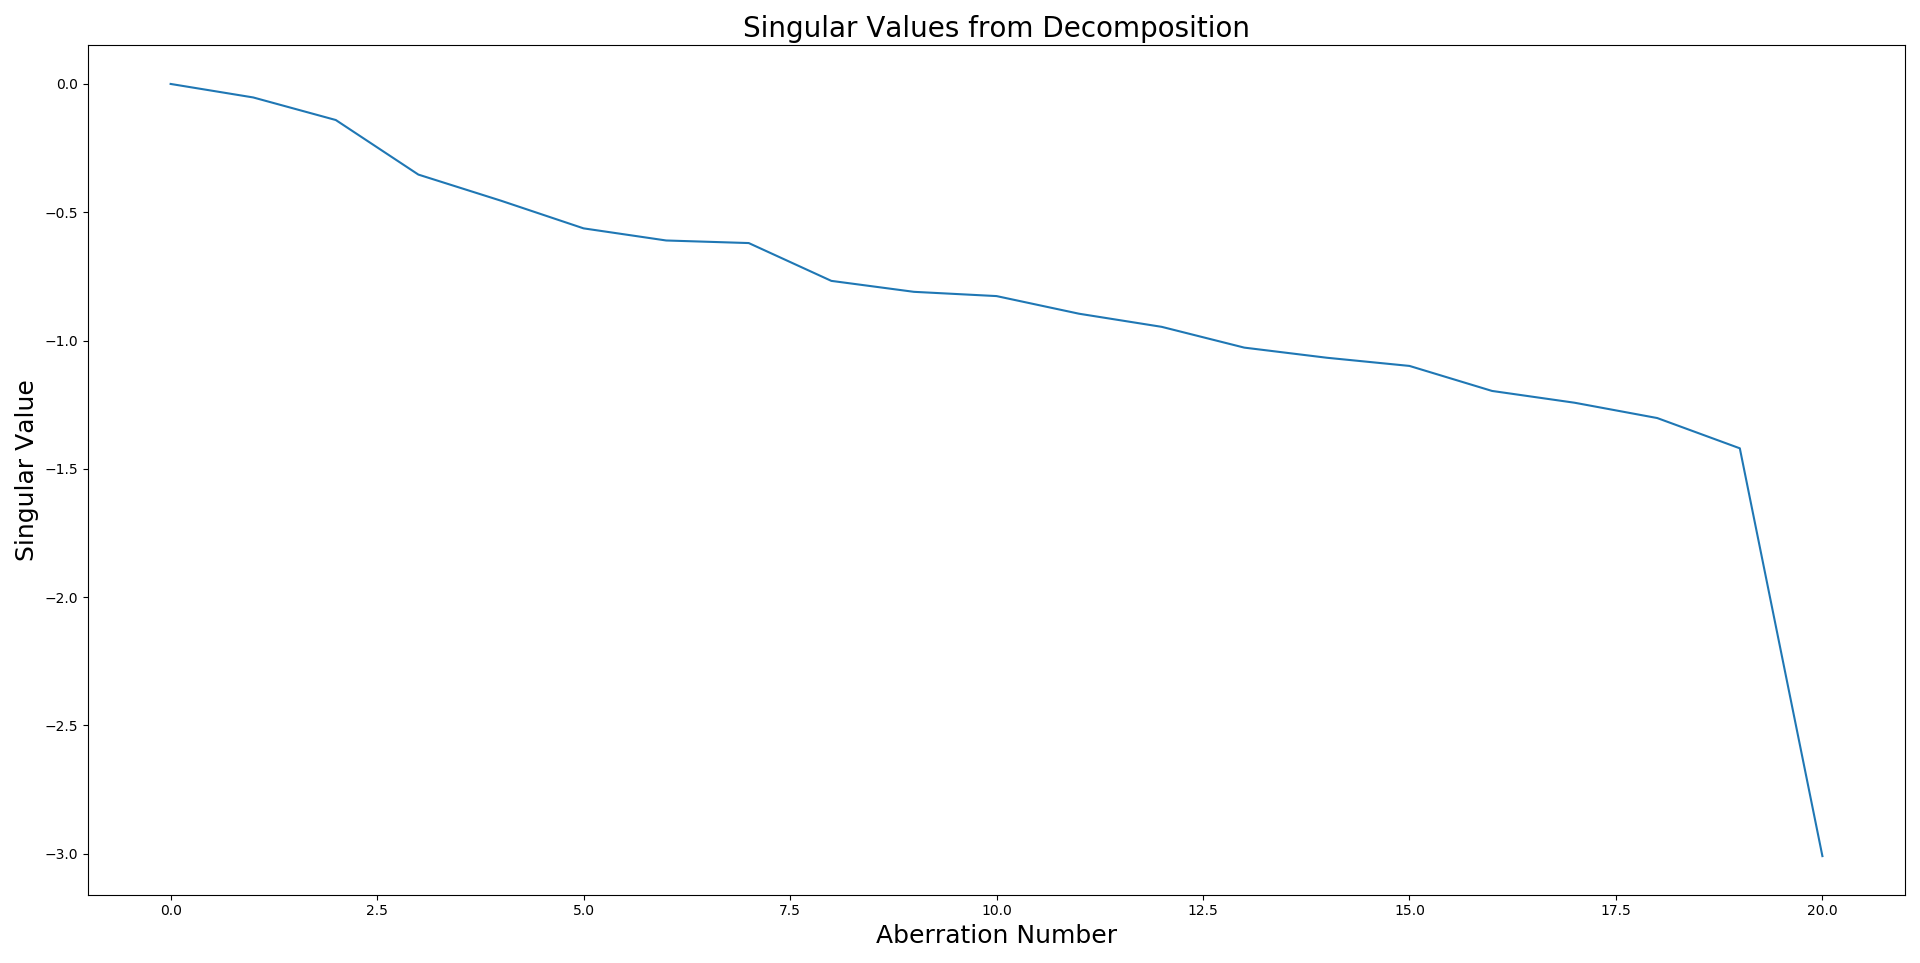
\includegraphics[width = 14cm]{Figures/singular_values.png}
    \caption{Singular Values of the Control Matrix.  There is a drop off in the singular value for mode 21.  This would normally be a cutoff point if the system was directly measuring Zernike modes.  However, since these modes are what the wavefront sensor is looking for, the last mode stays in the matrix.}
    \label{fig:SV}
\end{figure}


The singular values were confirmed to match previous versions of other response matrices made for the GMT.  Therefore, we could move on to testing the wavefront sensing ability of our system.  To test this, we first take a reference image of an unaberrated focal plane and subtract that from an aberrated image.  The left over image is a residual intensity between the two images.  With that image, we can take the dot product of the control matrix and the residual image to get the amplitudes of all the modal basis set.  The results of this will be discussed in Chapter \ref{Chapter4}.  Now that we have shown that we can do focal plane wavefront sensing with a vAPP, we can go on to physically demonstrating it.
 
% Chapter Template

\chapter{Optical Design} % Main chapter title
\noindent\textbf{\large Contents:}

\noindent\hrulefill
\noindent\startcontents[chapters]
\noindent\printcontents[chapters]{}{1}{}
\noindent\hrulefill
\label{Chapter3} % Change X to a consecutive number; for referencing this chapter elsewhere, use \ref{ChapterX}
% \tableofcontents

% \vspace{5mm}
This section will go over the process to come up with a new more manufactureable, optical design.  


\section{Mirror Systems}
\label{sec:mirror_sys}

The first option explored was to use mirror designs.  The use of mirrors has the 
added benefit of having zero photon loss.  As seen in Figure \ref{fig:reflect_diag}, the 
electric field of the system can be broken down into the incident electric field ($E^i$),
the reflected electric field ($E^r$) and the transmitted electric field ($E^t$).  Using conservation of energy we can get the following equation:
\begin{equation}
    E_0^i + E_0^r - E_0^t = 0
\end{equation}
With mirrors, the transmission component is zero, therefore the transmitted electric field
is equal to the incident electric field ($E_0^i = E_0^r$).  Mirrors also have the advantage of having more mechanical support since it is possible to mount mirrors on the back. 

\begin{figure}[h!]
\centering
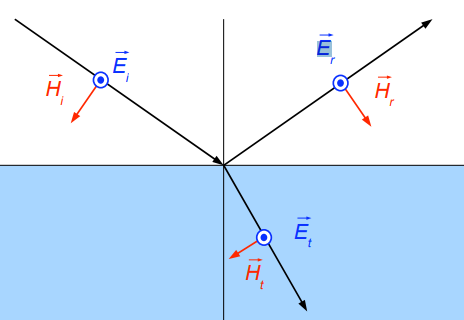
\includegraphics[width=8 cm]{Figures/reflection.png}
\caption{A diagram of the electric fields during the interaction with a medium \cite{keller_2019}.}
\label{fig:reflect_diag}
\end{figure}



The first
design looked at was using an Offner relay to zoom the pupil plane.  The design seen
in Figure \ref{fig:full_offner} was the resulting Offner relay.  The initial resulting
image (Figure \ref{fig:full_offner}), initially shows to have tilt in the image.  In ZEMAX
each field can have it's own color associated to it.  While it is not an exact indicator,
the change in color gives an approximation of the image plane.  This is because the
entrance pupil picks up the two fields at the same time, side by side.  So when the color
changes, this is representative of the two fields changing positions.

\begin{figure}[h!]
\centering
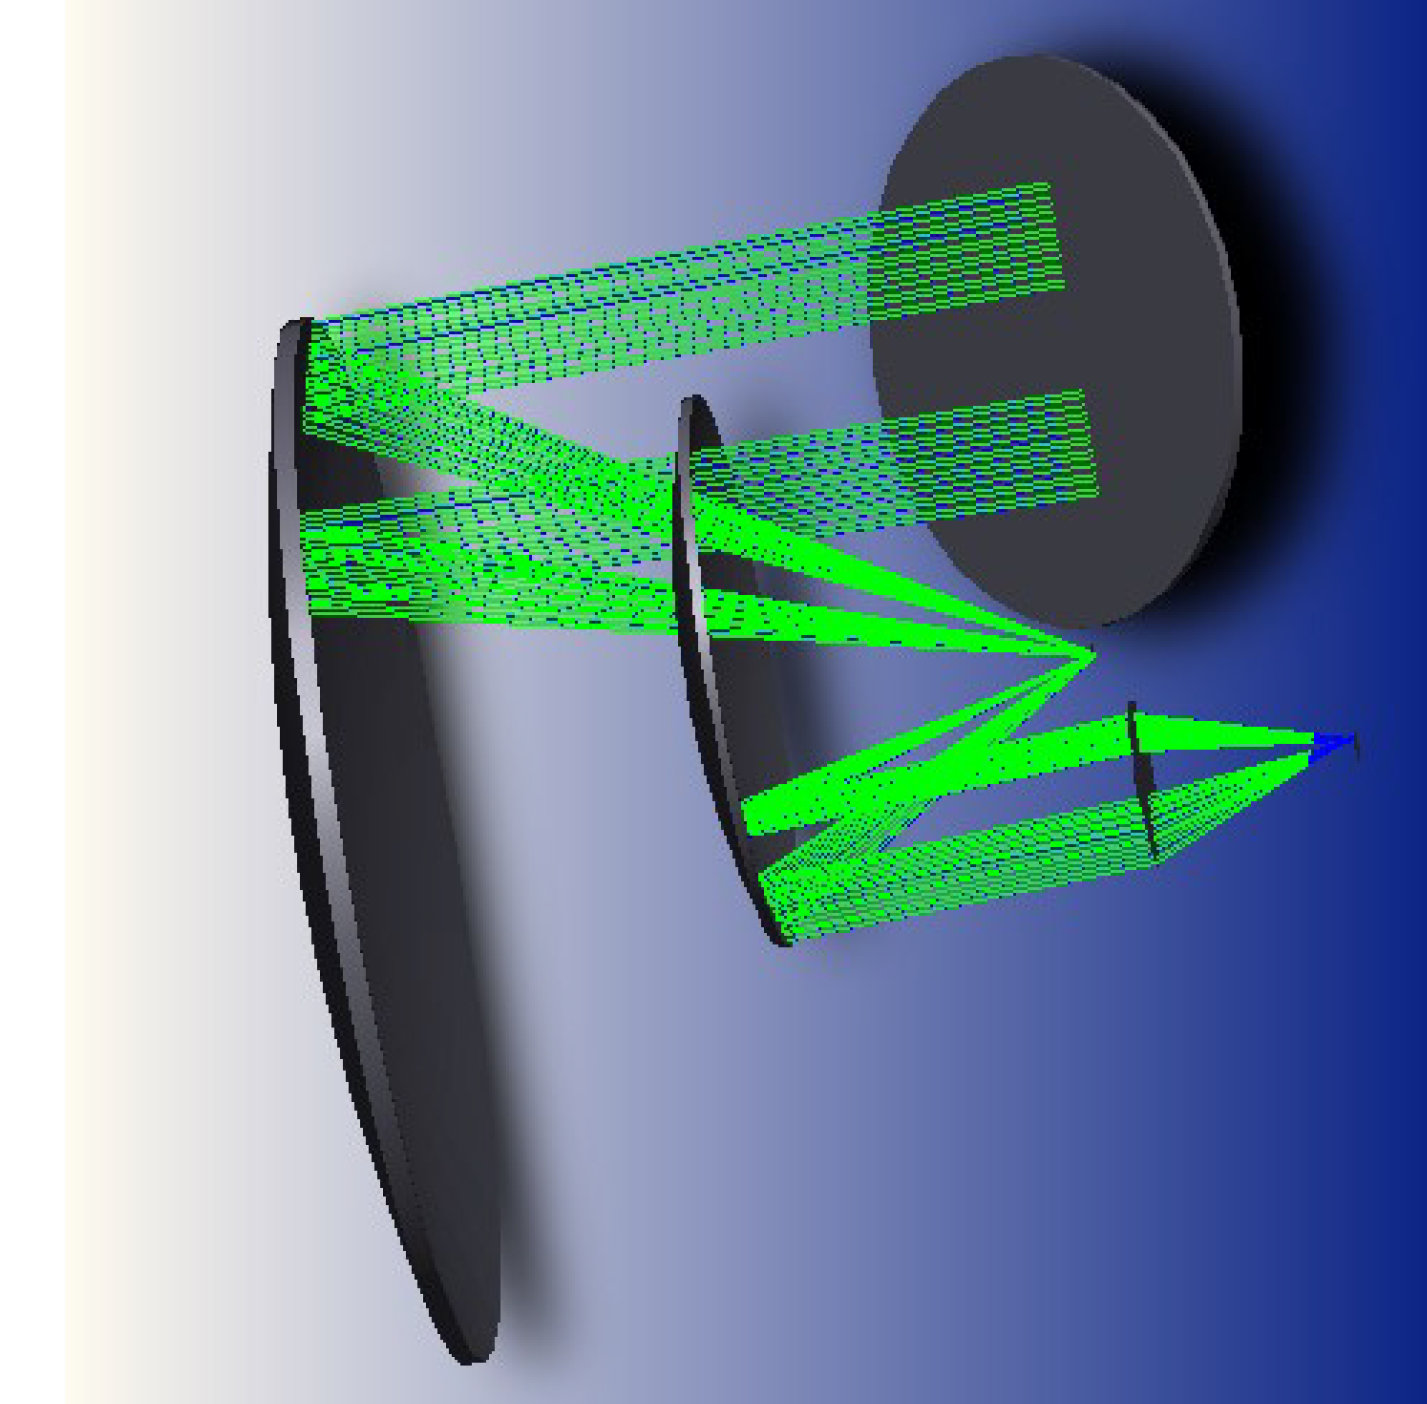
\includegraphics[width=8 cm]{Full_offner.png}
\caption{Above is the extent of the Offner Relay design.  The top right optic is the pick off mirror for the light coming from the laser.  From there the image has a 2x zoom by this configuration.  Note that for off-axis mirrors, ZEMAX constructs the entire mirror.}
\label{fig:full_offner}
\end{figure}

The motivation behind the Offner relay was that it was a simple way to zoom the 
pupil image while taking up the least amount of space.  However this soon became 
apparent that this design was not worth pursuing.  While Offner relays offer good
zoom depending on the placement of the mirrors, the change in focal length. In order
to correct for this, there would have to be additional optics to correct for this
since we want the pupil plane at the lenslet array to be as flat as possible.  These
additional optics would more than likely add to the physical dimension of the SLAO
system.  

\begin{figure}[h!]
\centering
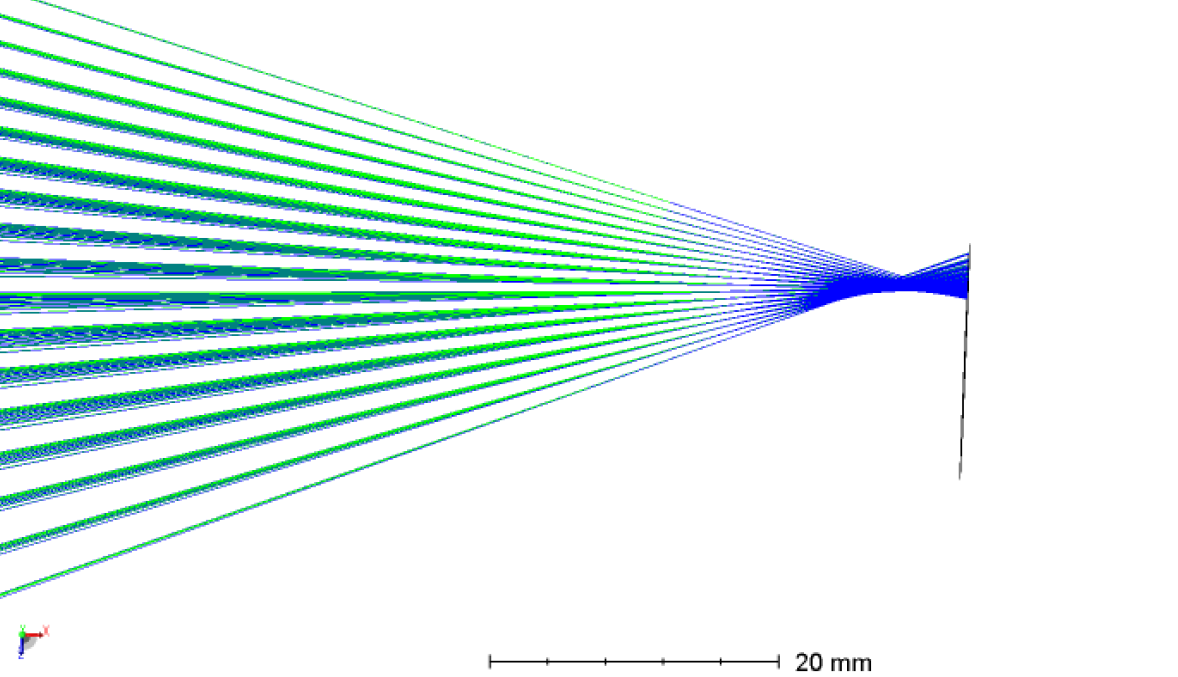
\includegraphics[width=14 cm]{offner_tilt.png}
\caption{An image of the first focus after the Offner relay zoom.  We can see that there is
significant tilt in the focal plane where the color change is.} % Explain this more
\label{fig:offner_tilt}
\end{figure}

Other designs were looked into, such as a Gregorian zoom system as well as off axis
parabolas in order to work in the space envelope.  But all showed similar issues
with space and tilt of the planes.  Because of this, going back to a full lens
system was deemed necessary and potentially simpler.  However, this required some 
design changes from the original design.  The original design had
three main lenses of varying size, all with aspherical surfaces.  The goal of this
design was to have an optical layout with all spherical surfaces.  Also due to
the fact that we are only dealing with one wavelength (595nm), the design could be
made with only one glass type.

\section{Optical Constraints}
\label{optical_constraints}

In order to redesign a new system from scratch, it is important to understand what
the system is supposed to do as well as what is constraining the system.  First
thing and maybe most importantly, is to focus the laser spot.  The laser spot is a
known distance from the telescope, therefore it will not be an infinity focus.  We
know that the sodium layer is roughly 90 km above sea-level with a approximate
thickness of 10 km \cite{sodium}.  So for the telescope pointing at Zenith, we can
assume that the laser spot is 90 km above the telescope.  As the telescope changes
zenith angle, the laser tracks the curvature of the Earth's atmosphere.  So the
distance of the laser spot can be computed as:

\begin{equation}
    d_{LGS} = \frac{z_{LGS}}{\cos \zeta}
\end{equation}

Where $d_{LGS}$ is the distance of the laser guide star (LGS), $z_{LGS}$ is the
distance at zenith, and $\zeta$ is the angle away from zenith.  The output of which
can be seen in Figure \ref{fig:laser_dist}.  With this information we can calculate
the difference in focal length between an object at infinity and the laser spot. 
First we take some approximations about the ELT itself:

\begin{enumerate}
    \item Diameter $(D) = 39m$
    \item $f/D = 17.48$
    \item $f = 681.72m$
\end{enumerate}

With this information we can do a first order approximation of where the focal point
of an object will be using a simple formula:

\begin{equation}
    \frac{1}{f} = \frac{1}{object} + \frac{1}{image} \;\;\;\; \rightarrow \;\;\;\; image = \left(\frac{1}{f} - \frac{1}{object}\right)^{-1}
    \label{eq:img_dist}
\end{equation}

\begin{figure}[h!]
\centering
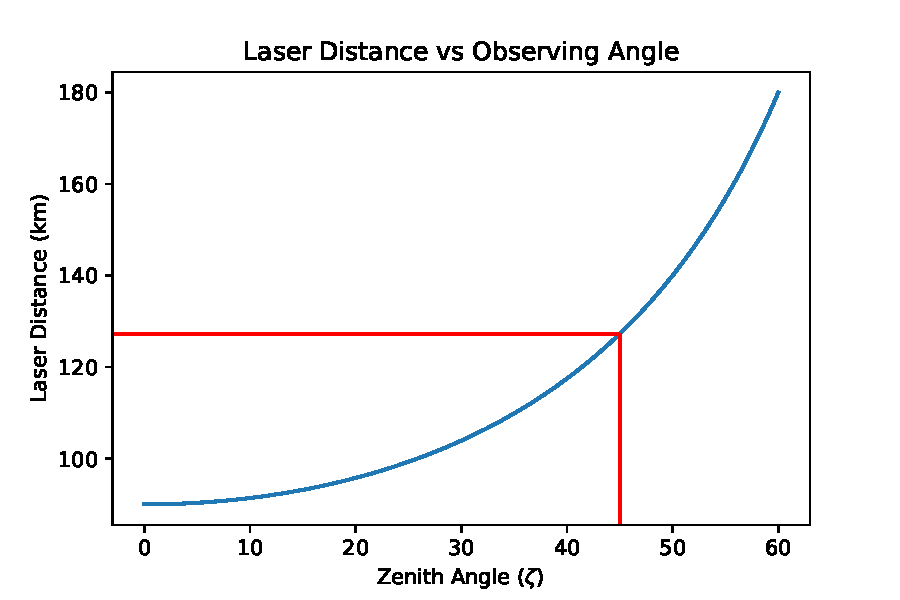
\includegraphics[width=10 cm]{Figures/las_dist.pdf}
\caption{A plot of laser distance versus Zenith angle.  The red lines mark the 45 degree zenith angle equaling a distance of 127km}
\label{fig:laser_dist}
\end{figure}

For an object at infinity, this equation simplifies to $image = f$.  Which in this
case means the image is approximately 682 meters behind the primary mirror.  This is
where the annular mirror mentioned in Chapter \ref{Chapter2} will be located.  Next
is to figure out how far back the laser light will focus.  Since we can assume that
the laser light will come to focus further than the science light, we can subtract
the distance by $682$ meters.  This can be visualized by Figure
\ref{fig:laser_focus}.

\begin{figure}[h!]
\centering
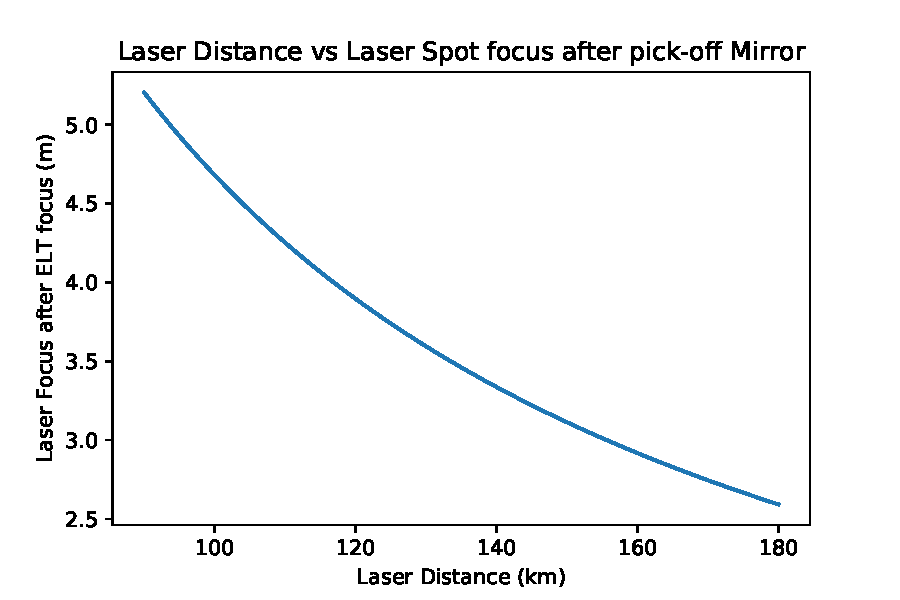
\includegraphics[width=10cm]{Figures/Laser_focus_vs_Laser_dist.pdf}
\caption{A plot of laser focal distance compared to the laser spot distance.  The focal length of the ELT is subtracted to show the distance between the annular mirror and the laser focus.}
\label{fig:laser_focus}
\end{figure}

\subsection{Lenslet Array Calculations}
\label{sec:lenslet_calc}
On the other side, we need to know what we are imaging.  First we note that the
camera chosen for this system is a Large vISble cAmera (LISA) chosen by ESO that has
a 800x800 pixel array with a pixel size of 24 microns.  This gives a total array
size of 19.2mm $\times$ 19.2mm \cite{SAPHIRA}.  The lenslet array will need to have
the following characteristics \cite{arcier}:

\begin{itemize}
    \item $40 \times 40$ subapertures
    \item 20 pixels per subaperture
    \item 10" FoV or 0.5" per pixel
\end{itemize}

The lenslet array needs to image directly onto the detector array to avoid any
aberrations in the pupil plane.  Therefore, the size of the lenslet array will need
to match the size of the detector array of 19.2mm.  The lenslet will subdivide the
pupil plane.  So each lenslet will cover an equivalent of $39m / 40 = 0.975 m$ of
the entrance pupil.  This gives a diffraction limit for each lenslet to be $\theta =
\lambda / d = 0.589\mu m / 0.975m = 0.124"$.  This gives the size of the Airy disk
for each lenslet of 0.124".  The pixel scale required is 0.5"/pixel.  This means
that the pixel size will be $\approx 4$ times the diffraction limit.  This means
that the pixel size needs to be $4 \times 0.589 \mu m = 2.4 \mu m$.  Since the pixel
size needs to be 24 microns, this means that the \textit{f}-number will need to be
equal to 10.  The diameter of each of these lenslets will be $19.2mm / 40 = 0.48mm$.
Since we know what the speed of the lenslet should be, we can calculate the focal
length of each lenslet:

\begin{equation}
    f/D = N \;\;\;\; \rightarrow \;\;\;\; f = N \times D = 10 \times 0.48mm = 4.87mm
\end{equation}

The key characteristics of the lenslet array are as follows:

\begin{itemize}
    \item $f = 4.87mm$
    \item $D = 0.48mm$
    \item $40 \times 40$ array
\end{itemize}


\subsection{Design of First Lens}
\label{sec:L1_des}
Referring back to Chapter \ref{Chapter2} again, we don't want to a system that is
almost 5 meters long just to have the light come to focus.  It is important that the
first optic accelerate the light convergence in order to save space.  For simplicity
sake, we place our first lens one meter away form the annular mirror.  We want the
lens to have an F-number of roughly 3 ($f/D = 3$).  So in order to do this, it was
first necessary to find the diameter of the lens one meter away from the annular
mirror.  The laser spot size is the largest when the telescope is at zenith,
therefore the calculations for this will be done at $\zeta = 0$. I wrote a small
code to determine the size of L1 based on the focal length of the laser and the
speed of a system.  This uses the simple equation $f/D = N$ to determine $D$ based
on a distance behind the focal point.

\begin{lstlisting}
def find_D(D,N,f1,f2):
    dist_new = f1 - f2
    D_new = dist_new / N
    return D_new
    
D_L1 = (find_D(D_ELT,N_ELT,laser_focus[0],dist_to_L1)).to(u.cm)
print(D_L1)

24.04584882426677 cm
\end{lstlisting}

This returned a diameter of 24 cm and from this we can calculate what the focal
length of Lens 1 (L1) should be $f/D = N \; \rightarrow \; f = N \times D = 3 \times 24.05cm
= 72.1 cm$.  With this focal length established, next is to find where the pupil
plane is located and where the focal point is after L1.
\label{op_L1}

\subsection{The Rest of the System}
\label{sec:sys_require}

With the constraints explained in Section \ref{optical_constraints} and Section
\ref{op_L1}, the rest of the system has a very straight forward approach to
calculating the variables of each optic.  First, we calculate the conjugate planes
after L1.  We can do this by using Equation \ref{eq:img_dist} and the output from
Figure \ref{fig:laser_dist}.  

We also want to know where the pupil plane is.  Instead of taking the distance to
the entrance pupil of ELT, we will use the distance from the exit pupil of the ELT.
The exit pupil is defined as "the image of the aperture stop as seen from an axial
point on the image looking through the interposed lenses \cite{Hecht}."  Here the
aperture stop is the primary mirror the ELT itself.  According to ZEMAX, the exit
pupil is located 38.349 meters away from L1.  Since this location does not change
with zenith angle, this distance will stay the same.  The output of these different
planes can be seen in Figure \ref{fig:L1}


\begin{figure}[h!]
\centering
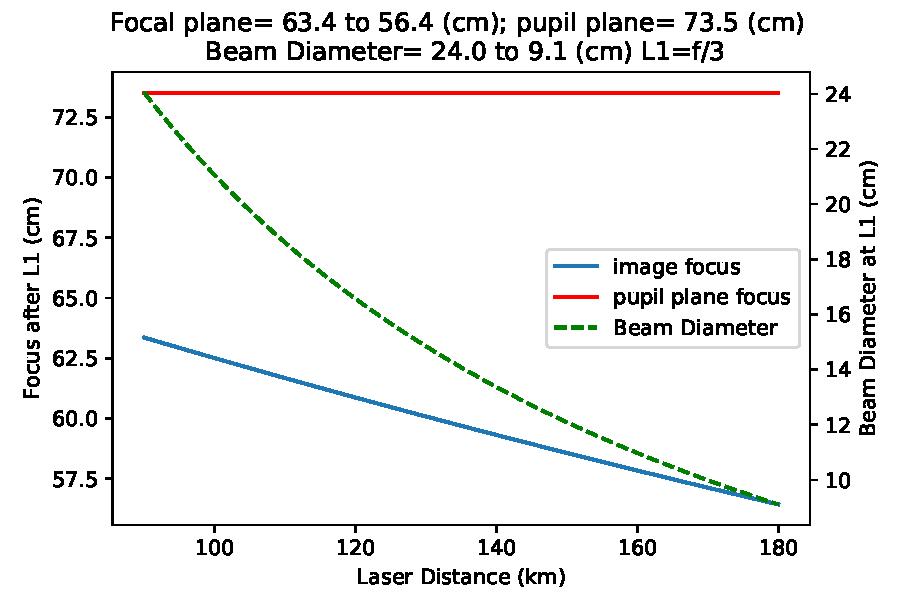
\includegraphics[width=14 cm]{Figures/L1_dim.pdf}
\caption{A plot of the different characteristics of L1.  Note that the pupil plane is constant.}
\label{fig:L1}
\end{figure}

Next (yes you guessed it) comes L2.  L2 needs to focus the pupil plane to infinity.
This is done by locating L2 one focal length away from the pupil plane.  The reason
the pupil plane should be focused to infinity is that the focal plane still varies
in distance with respect to zenith angle.  In the space between L2 and the next
optic, L3, there can be an altitude compensator without impacting the image quality
of the pupil plane.  The focal length of L2 was not so fixed as the rest of the
system.  A few different focal lengths were tested and the output of which can be
seen in Figure \ref{fig:L2}.

In Figure \ref{fig:L2}, there are a range of options for the focal length of L2. 
The choice came down to two factors: 1) The speed of the system, and 2) linearity. 
A focal length of 12.5 cm was deemed a good choice since it gave a f-number of 1.25,
which is slow enough not to add too many aberrations and quick enough to make the
system more compact, and the linearity of the range of focus is a nice thing to
have.  

\begin{figure}[h!]
\centering
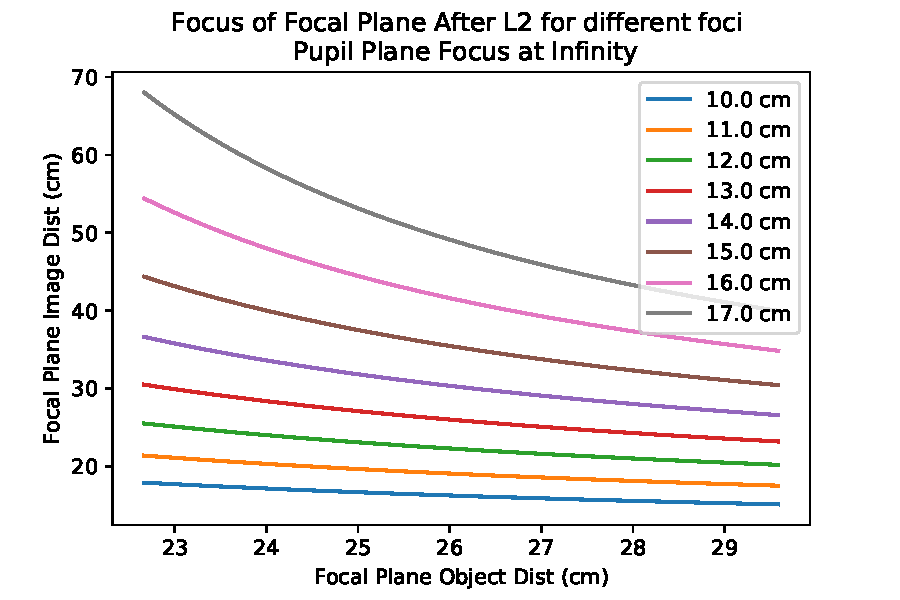
\includegraphics[width=14 cm]{Figures/L2_varying_focus.pdf}
\caption{A plot of the back focal distances of the laser spot after L2 with the focal 
length of L2 listed in the legend.}
\label{fig:L2}
\end{figure}

The rest of the system was designed to do two things: 1) pass the light to a beam
size that matches the size of the lenslet array, 2) and then create a telecentric
lens that focuses the pupil image onto the lenslet array.  Telecentricity is an 
optical property that has the pupil image suffer only from defocus and does not 
suffer from demagnification.
%Silly humor, not sure how well it will go over.  May delete
% With these constraints in place and understood, the next step is.  Not quite the case.  To begin withd, a first order must be put in place.  
The next step is to create an optical drawing of the system.  Before looking into
manufacturable optics, we can make an ideal approximation using a paraxial lens.
The paraxial design was first drawn up (Figure \ref{fig:paraxial_draw}) and then
inserted into ZEMAX.

\begin{figure}[h!]
\centering
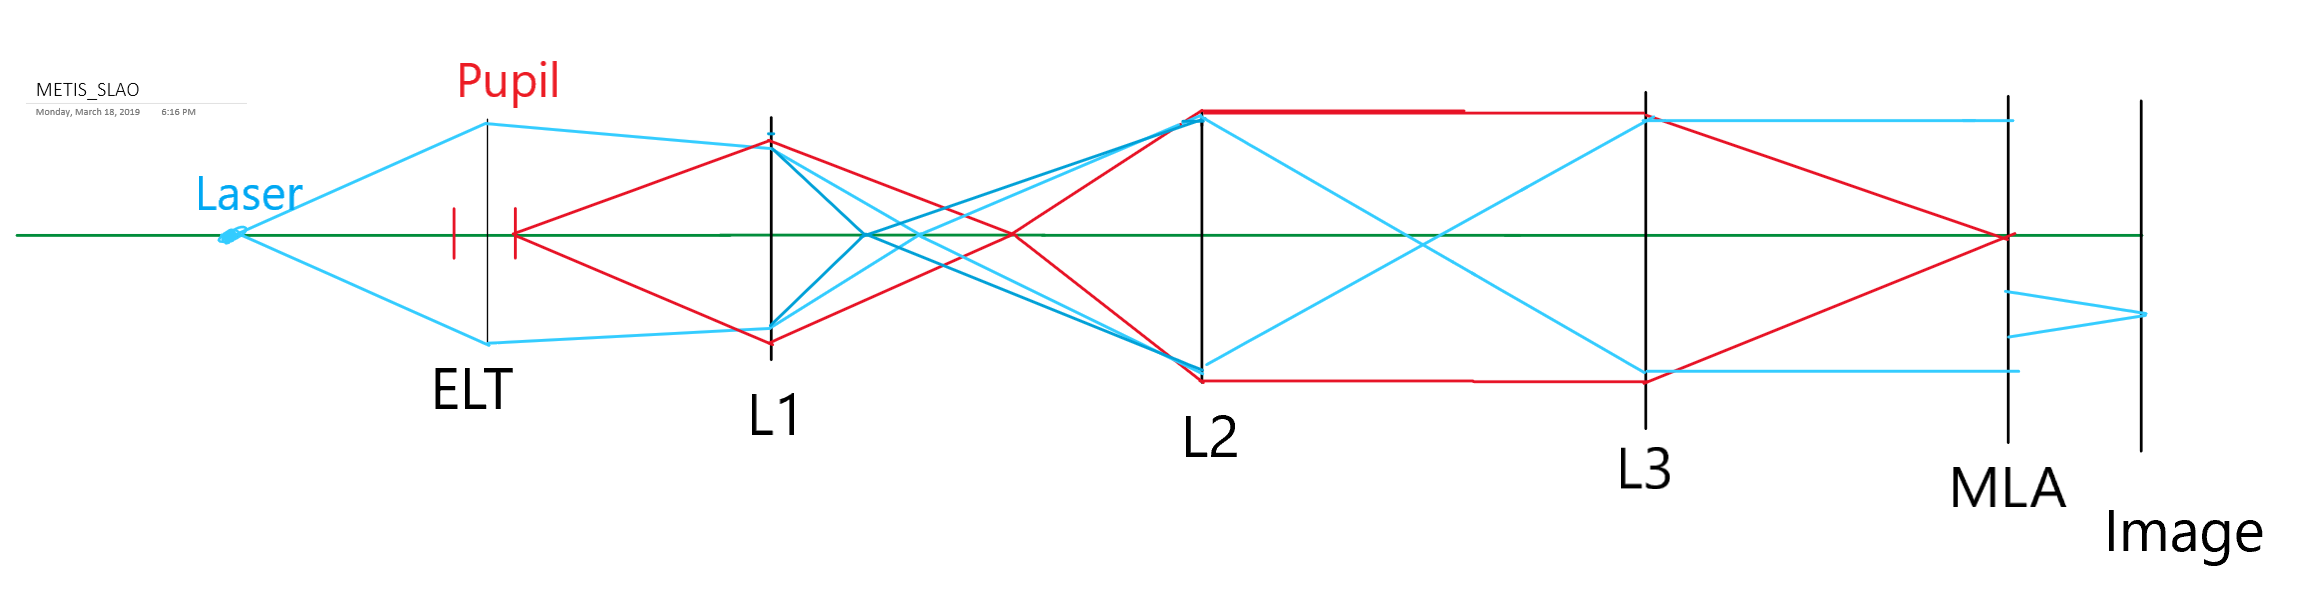
\includegraphics[width=14 cm]{Figures/paraxial_draw.png}
\caption{A drawing of the paraxial design.  Note that after L2 the focus of the pupil is at infinity.}
\label{fig:paraxial_draw}
\end{figure}

\section{Realistic Design}
\label{sec:reality}

Here I go through the steps necessary to reach a manufacturable optical system.

\subsection{Paraxial Design}
\label{sec:real_paraxial}

A paraxial approximation is another version of the small angle approximation, where
a ray angle $\theta \approx \tan \theta$ \cite{greivenkamp_2004}.  More simply put,
this is the approximation of an ideal lens with no thickness and no radius of
curvature, just a focal length.  With the data from Section
\ref{optical_constraints}, we can make a table of each lenses attributes as seen in
Table \ref{tab:lens_data}.  Next, the data is applied into to get Figure
\ref{fig:paraxial_layout}.


\begin{table}[h!]
\begin{tabular}{|c|c|c|c|c|}
\hline
\textbf{Objecet} & \textbf{$f$} & \textbf{Lens Diameter} & \textbf{Distance to next object} & \textbf{N} \\ \hline
\textbf{L1}      & 72.1 cm      & 24 cm                  & 86 cm                            & 3          \\ \hline
\textbf{L2}      & 12.5 cm      & 10 cm                  & varying                          & 1.25       \\ \hline
\textbf{L3}      & 15 0mm        & 50 mm                   & 100 mm                            & 3          \\ \hline
\textbf{Tele}    & -60 mm        & 19.2mm                 & 0                                & -          \\ \hline
\textbf{LA}      & 4.87 mm       & 19.2 mm                 & 4.87 mm                           & 10         \\ \hline
\end{tabular}
\caption{Table of key dimensions of the SLAO system.  For simplicity sake, the distance between the telecentric lens and the lenslet array is 0 in ZEMAX.}
\label{tab:lens_data}
\end{table}

\begin{figure}[h!]
\centering
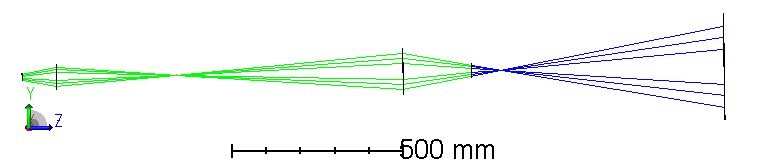
\includegraphics[width=14 cm]{Figures/paraxial_layout.png}
\caption{Paraxial layout of the built system.}
\label{fig:paraxial_layout}
\end{figure}

\subsection{Realistic System}
\label{sec:Optical_real}

With the paraxial system in place, next was to introduce optics that had the same
characteristics as the paraxial lens.  ZEMAX has a built in function that will allow
a user to input a diameter and a focal length and will find an off-the-shelf part to
match your specification.  When inserting a manufacturable lens into ZEMAX, there are a few
parameters that make up a basic lens:

\begin{enumerate}
    \item Radius of curvature
    \item Thickness
    \item Material
\end{enumerate}

Zemax has the user build a surface based off of these parameters.  A lens is made up
of two surfaces (Figure \ref{fig:real_lens}).  With the introduction of more
physical lenses, image quality and pupil quality.  The next step is to construct a
proper merit function to constrain the system and let the program optimize itself.


\begin{figure}[h!]
\centering
\begin{subfigure}{.5\textwidth}
  \centering
  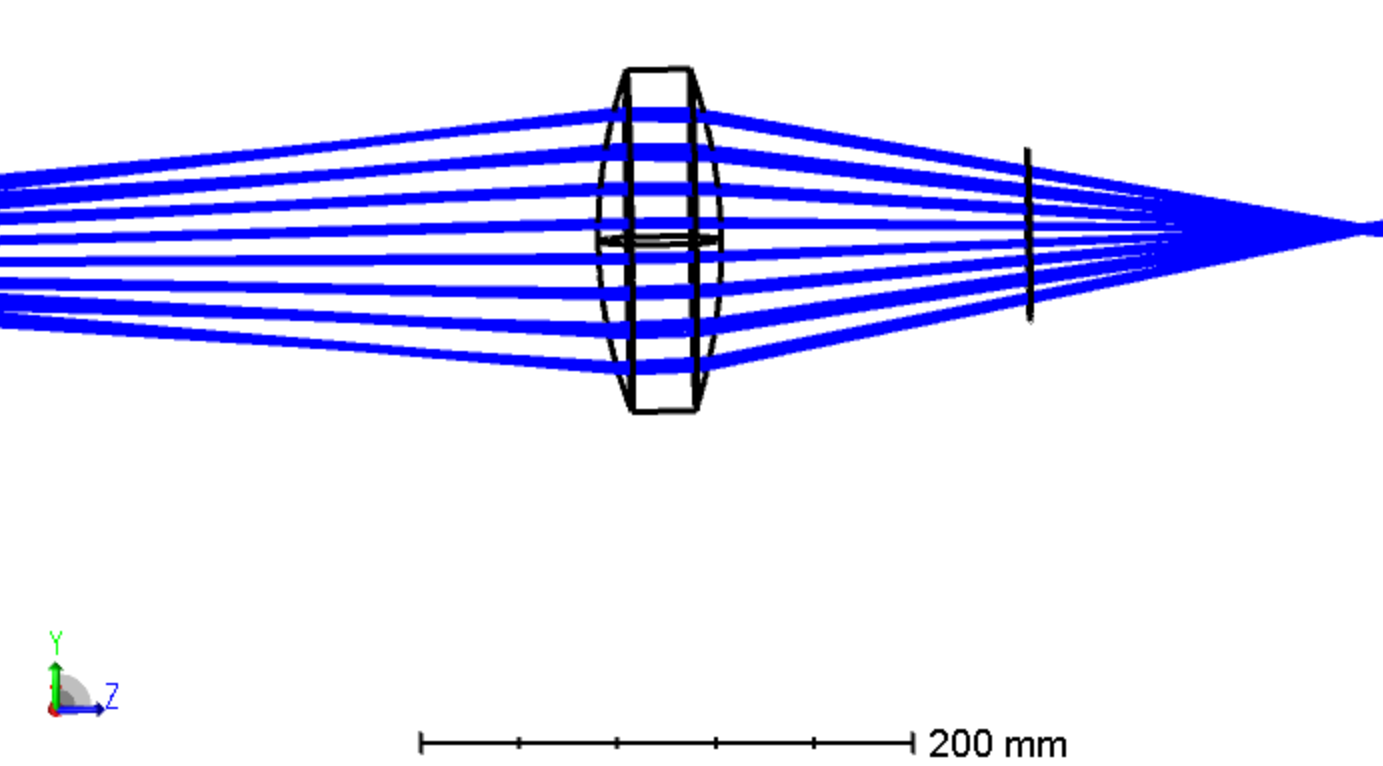
\includegraphics[width=6cm]{Figures/real_lens.png}
  \caption{An example of what a lens looks like in ZEMAX}
  \label{fig:real_lens}
\end{subfigure}%
\begin{subfigure}{.5\textwidth}
  \centering
  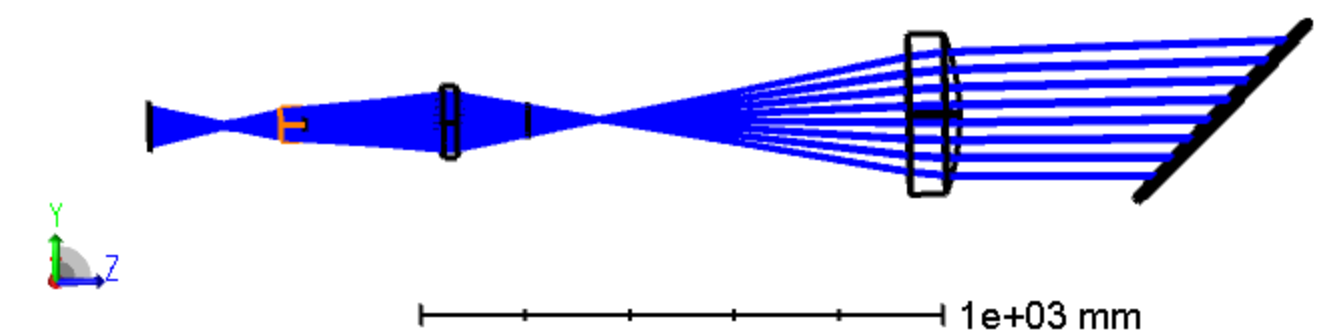
\includegraphics[width=6cm]{Figures/real_system_1.png}
  \caption{Figure of the same system with real lenses.}
  \label{fig:lens_system_1}
\end{subfigure}
% \caption{}
\label{fig:real_1}
\end{figure}


\subsection{Adding additional lenses}
\label{sec:real_more_lens}

Since the design was not working with substituting single lenses for paraxial ones,
the next idea was to divide a single lens into two lenses by inserting two surfaces
in the middle of a lens.  This would allow ZEMAX to have additional variables at its
disposal to better optimize the system.  An example can be seen in Figure
\ref{fig:2x_lens}.


\begin{figure}[h!]
\centering
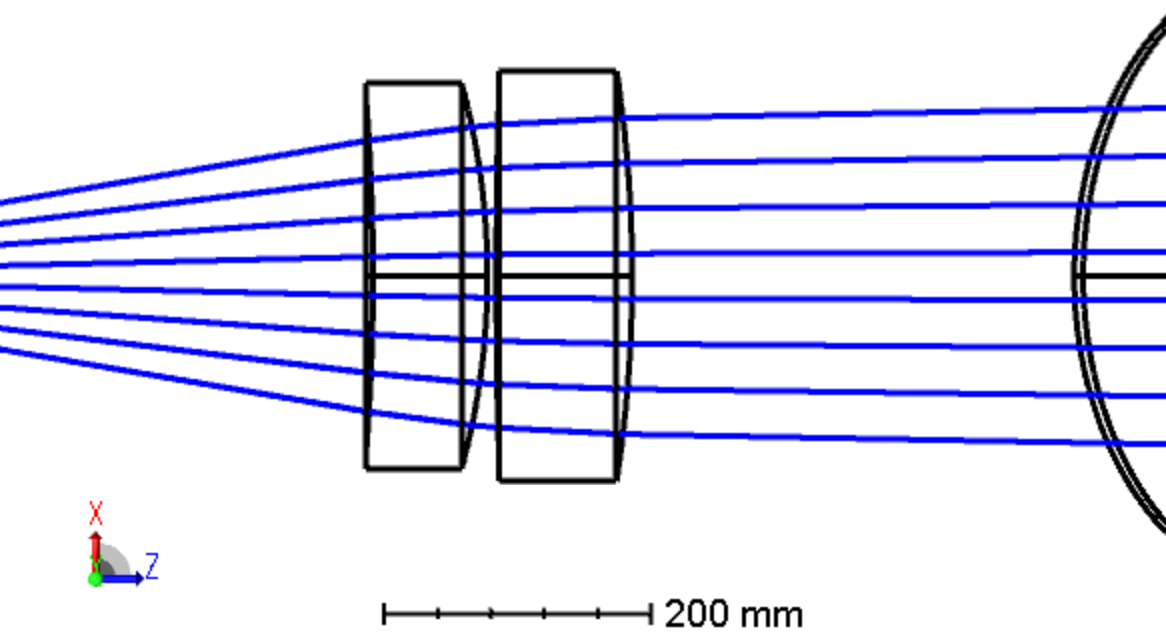
\includegraphics[width=12cm]{Figures/2x_L1.png}
\caption{An Example of splitting a lens into two different optical components.}
\label{fig:2x_lens}
\end{figure}

Now that the system has become more complicated, there needs to be more constraints
on the system.  ZEMAX, like most software, will not always do what you want it to at
first.  Unless otherwise specified, ZEMAX has no issue creating lenses inside of
lenses and creating negative space in order to achieve the performance specified. 
As my advisor Remko Stuik said, "there are a million different ways that an
optimization can go wrong, but only one way for it work correctly."  The way to
correctly optimize a system in ZEMAX is to build a merit function. There are a few
things the Merit function was crucial in.  First, the merit function allows the user
to prevent unrealistic designs such as lenses within lenses and negative
thicknesses.  Second, it also allows you to place pupil and focal planes in certain
locations.  This was a crucial aspect of this design since the lenslet array needs
to image the pupil plane.  That means the pupil plane needs to land exactly on the
face of the lenslet array.  Lastly, the spot size.  It is possible to have a system
with excellent pupil quality.  However, if the spot size is not diffraction limited
then the system cannot provide accurate wavefront measurements.


\begin{figure}[h!]
\centering
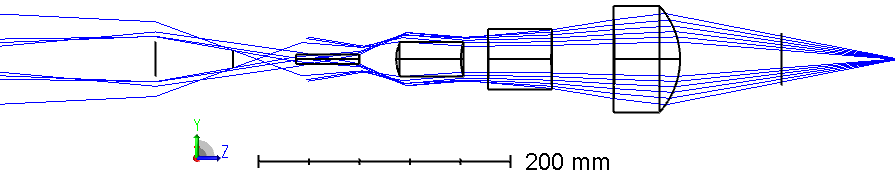
\includegraphics[width=14cm]{Figures/wo_merit_function.png}
\caption{An Example of how a system can "blow up" without the correct Merit Function.}
\label{fig:wo_merit}
\end{figure}

With a proper Merit function, designing a proper system was just an iterative
process of optimizing, patience, understanding what had changed, and what function
was driving those changes.  After optimization, the system was not providing an
acceptable wavefront in the pupil plane.  The next step was to find where an aspherical
surface could be located in order to provide the desired performance.  This goes in
contrast of the original goal of this thesis.  Originally, the system was to have no
aspherical lenses.  However, having one aspherical surface could prove to be cheaper than
adding additional optics that require space, and mounting.  ZEMAX has a feature called
"Find Best Asphere", where it goes through each optical surface and attempts to drive the
Merit Function as low as possible.  While running through the whole system would be a
definitive way to determine the best surface, a close look at the system can show where the
best surface would be (Figure \ref{fig:good_pupil}).


\begin{figure}[h!]
\centering
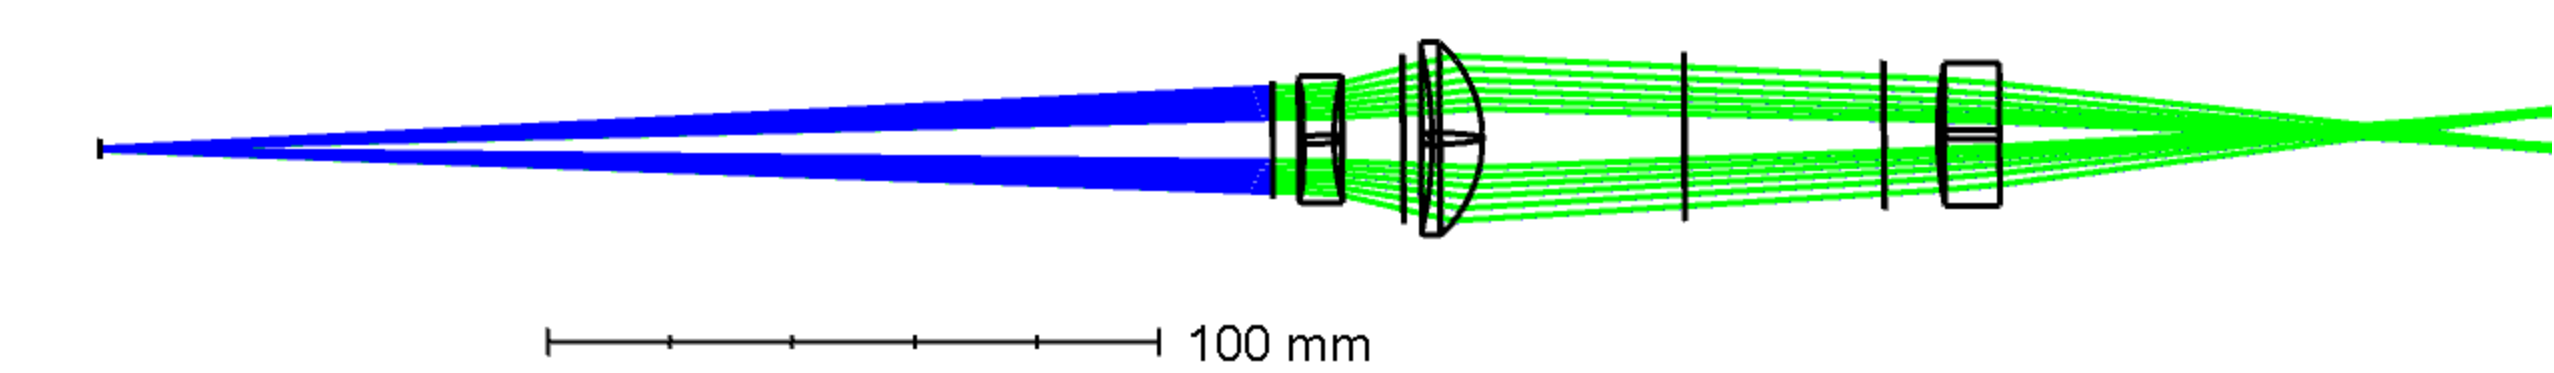
\includegraphics[width=14cm]{Figures/good_pupil.png}
\caption{An image of the last few optics in the system.  Where the color changes from green to blue is a rough indicator of where the pupil plane is.}
\label{fig:good_pupil}
\end{figure}

In Figure \ref{fig:good_pupil}, we can see where the pupil plane is.  Here there is
still a paraxial representation of the lenslet array.  At this location there is
still high wavefront error.  The surface just before the lenslet array would be the
ideal candidate.  If the asphere could match the wavefront error, then there would
be a flat wavefront reaching the lenslet array.  To be safe, ZEMAX ran through each
surface in Figure \ref{fig:good_pupil} to determine which was the best asphere.  The
back of the telecentric lens was indeed the best candidate.  From that the inline
design optimized to reduce the Peak-to-Valley (PTV) wavefront and drive the spot
size down to the diffraction limit.

The design shown in Figure \ref{fig:full_lens} showed that a design could be made to
accurately do wavefront sensing with only one aspherical surface.  The next step was
to implement a simpler way to extend the light path for the changing laser distance.

\begin{figure}[h!]
\centering
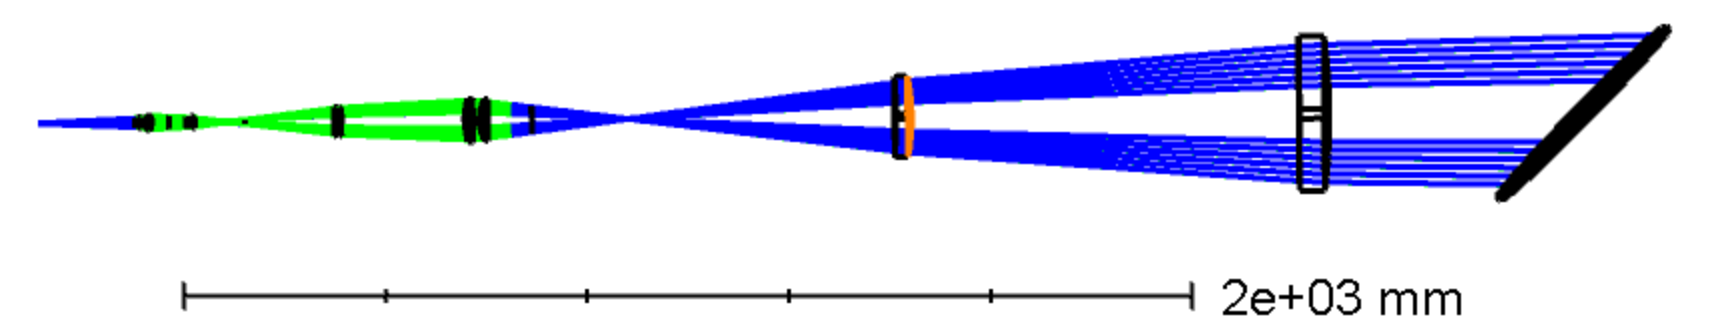
\includegraphics[width=14cm]{Figures/full_lens.png}
\caption{A layout of the in line WFS.}
\label{fig:full_lens}
\end{figure}


First, it is important to know where the light path can be extended without effect
system performance.  The pupil image quality is what needs to be preserved.  Going
back to Figure \ref{fig:paraxial_draw}, we can see that the pupil image is focused
to infinity between L2 and L3.  This is where the system can correct for the
changing laser distance.  When looking at concepts to compensate for the changing
altitude, we look to other instruments going onto the ELT.  HARNOMI impliments a
telescoping mirror system to extend the light path as seen in Figure
\ref{fig:harmoni}.

\begin{figure}[h!]
\centering
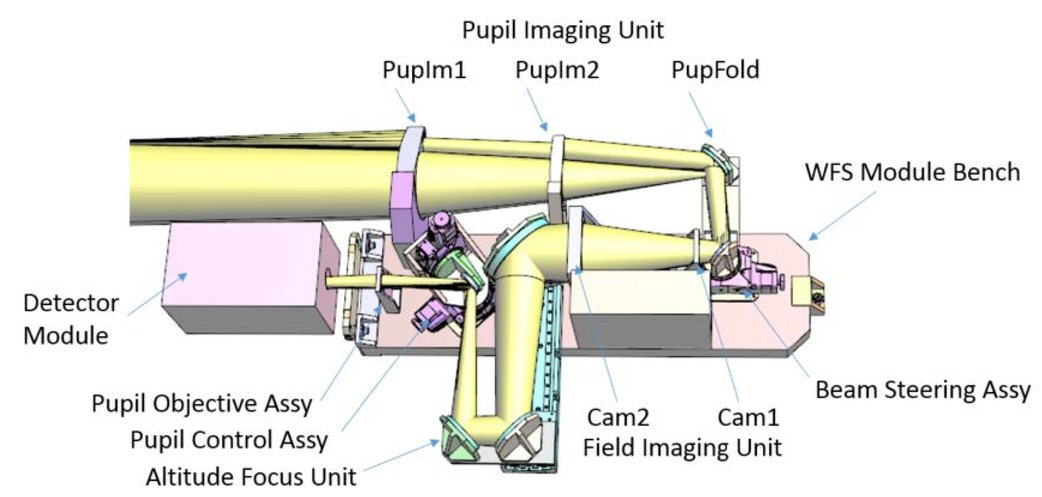
\includegraphics[width=14cm]{Figures/HARMONI_AO.jpg}
\caption{A layout of the HARMONI WFS.  In here the use a telescoping mirror system labeled as Altitude Focus Unit \cite{harmoni}.}
\label{fig:harmoni}
\end{figure}

A similar system was implemented in the design of the METIS SLAO system.  This meant
extending the distance between L2 and L3.  However, with a stable merit function,
this was easily implemented (Figure \ref{fig:SLAO_comp}).

\begin{figure}[h!]
\centering
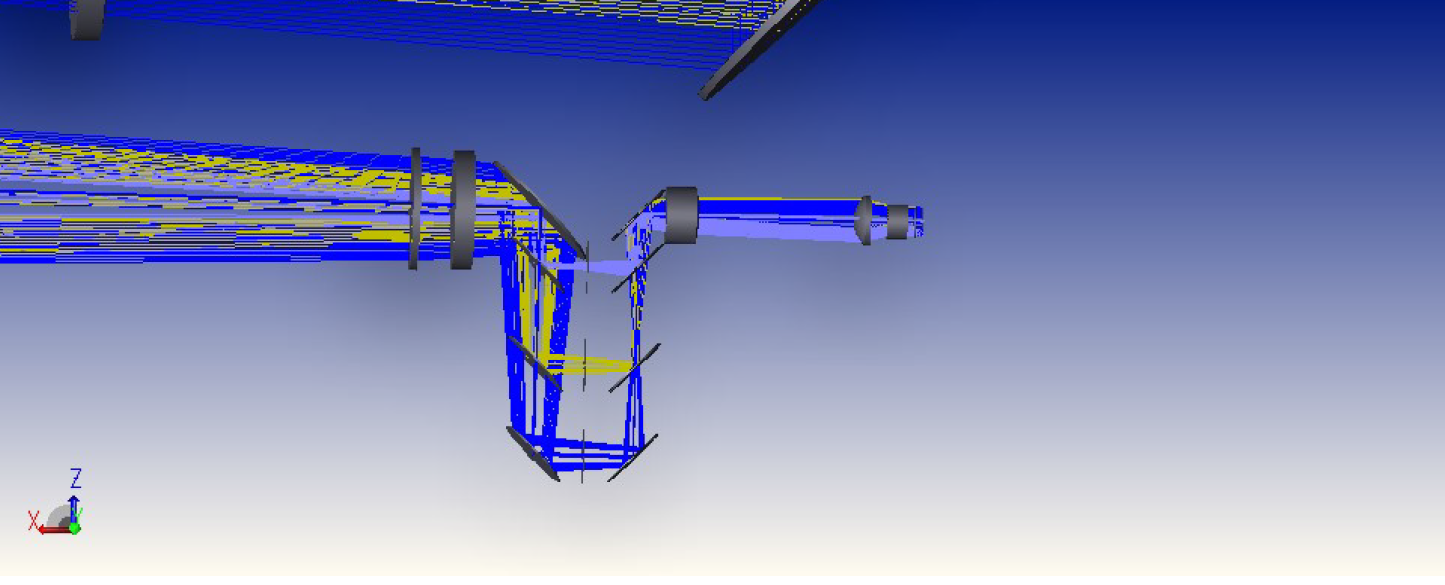
\includegraphics[width=14cm]{Figures/shaded_zoom.png}
\caption{A layout of the METIS SLAO altitude compensator.}
\label{fig:SLAO_comp}
\end{figure}

Next, the system needed to be more compact.  One of the requests of the METIS SLAO
system was to make the structure as compact as possible.  The simplest way to
achieve this was to add $45^{o}$ fold mirrors in between the lenses.  Flat, $45^{o}$
mirrors only create coordinate changes, but do not effect the image quality.  By
adding the fold mirrors, the almost 3 meter long system was reduced to less than a
meter long.  The full system with fold mirrors and altitude compensator can be seen
in Figure \ref{fig:SLAO_trace}.

\begin{figure}[h!]
\centering
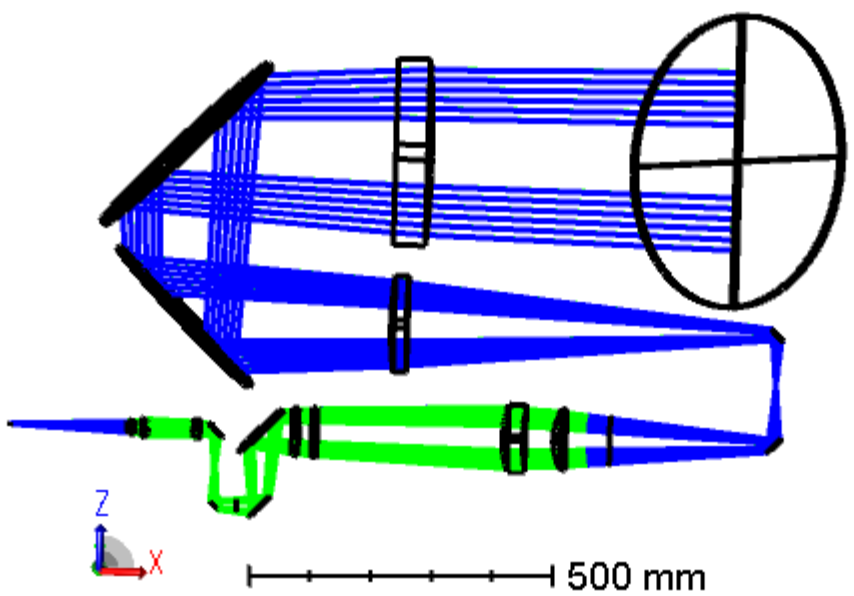
\includegraphics[width=14cm]{Figures/system_trace.png}
\caption{A layout of the full METIS SLAO design.}
\label{fig:SLAO_trace}
\end{figure}

The last step was to replace the paraxial lenslet array.  With the spot size and
wavefront within tolerance, it was time to substitute in a realistic lenslet array.
Adding a lenslet array into ZEMAX can be done multiple ways.  Normally ZEMAX allows
for a non-sequential component to be added into a sequential system.  The way to do this
in ZEMAX is to select "Non-sequential Component" in the "Surface Type" section.  From this
you can open up the "Non-sequential Component Editor".  In this you can normally add as
many non-sequential components as you'd like.  From there, an exit port surface needs to be
made in order for ZEMAX to go back to calculating sequentially\cite{zemax_non_seq}. 
Despite making practice files and making them work outside of the system, it continued to
fail when attempting to add it to the layout.

The next way was to use a "User Defined" surface.  This option allows for the
creation of a lenslet array in a sequential manner.  However, this method does not
allow for stable optimization in ZEMAX.  The output from a lenslet array is of
course, an array of spots.  ZEMAX wants to have all of the rays through a pupil
converge into one spot.  Therefore, optimization was not an option.  Using the
calculations from \ref{sec:lenslet_calc}, a lenslet array was designed from these
parameters.  From there, I used the slider function in ZEMAX to nudge the image
plane after the lenslet array into focus.  With the design in place, we can begin to
look at the kind of performance it will achieve.

\chapter{Results of Optical Design} % Main chapter title
\noindent\textbf{\large Contents:}

\noindent\hrulefill
\noindent\startcontents[chapters]
\noindent\printcontents[chapters]{}{1}{}
\noindent\hrulefill
\label{Chapter4}

 
\chapter{Conclusion} % Main chapter title
 

%----------------------------------------------------------------------------------------
%	THESIS CONTENT - APPENDICES
%----------------------------------------------------------------------------------------

\appendix % Cue to tell LaTeX that the following "chapters" are Appendices

% Include the appendices of the thesis as separate files from the Appendices folder
% Uncomment the lines as you write the Appendices

% Appendix A

\chapter{Wavefront Maps} % Main appendix title

\label{AppendixA} % For referencing this appendix elsewhere, use \ref{AppendixA}

\begin{figure}[h!]
\centering
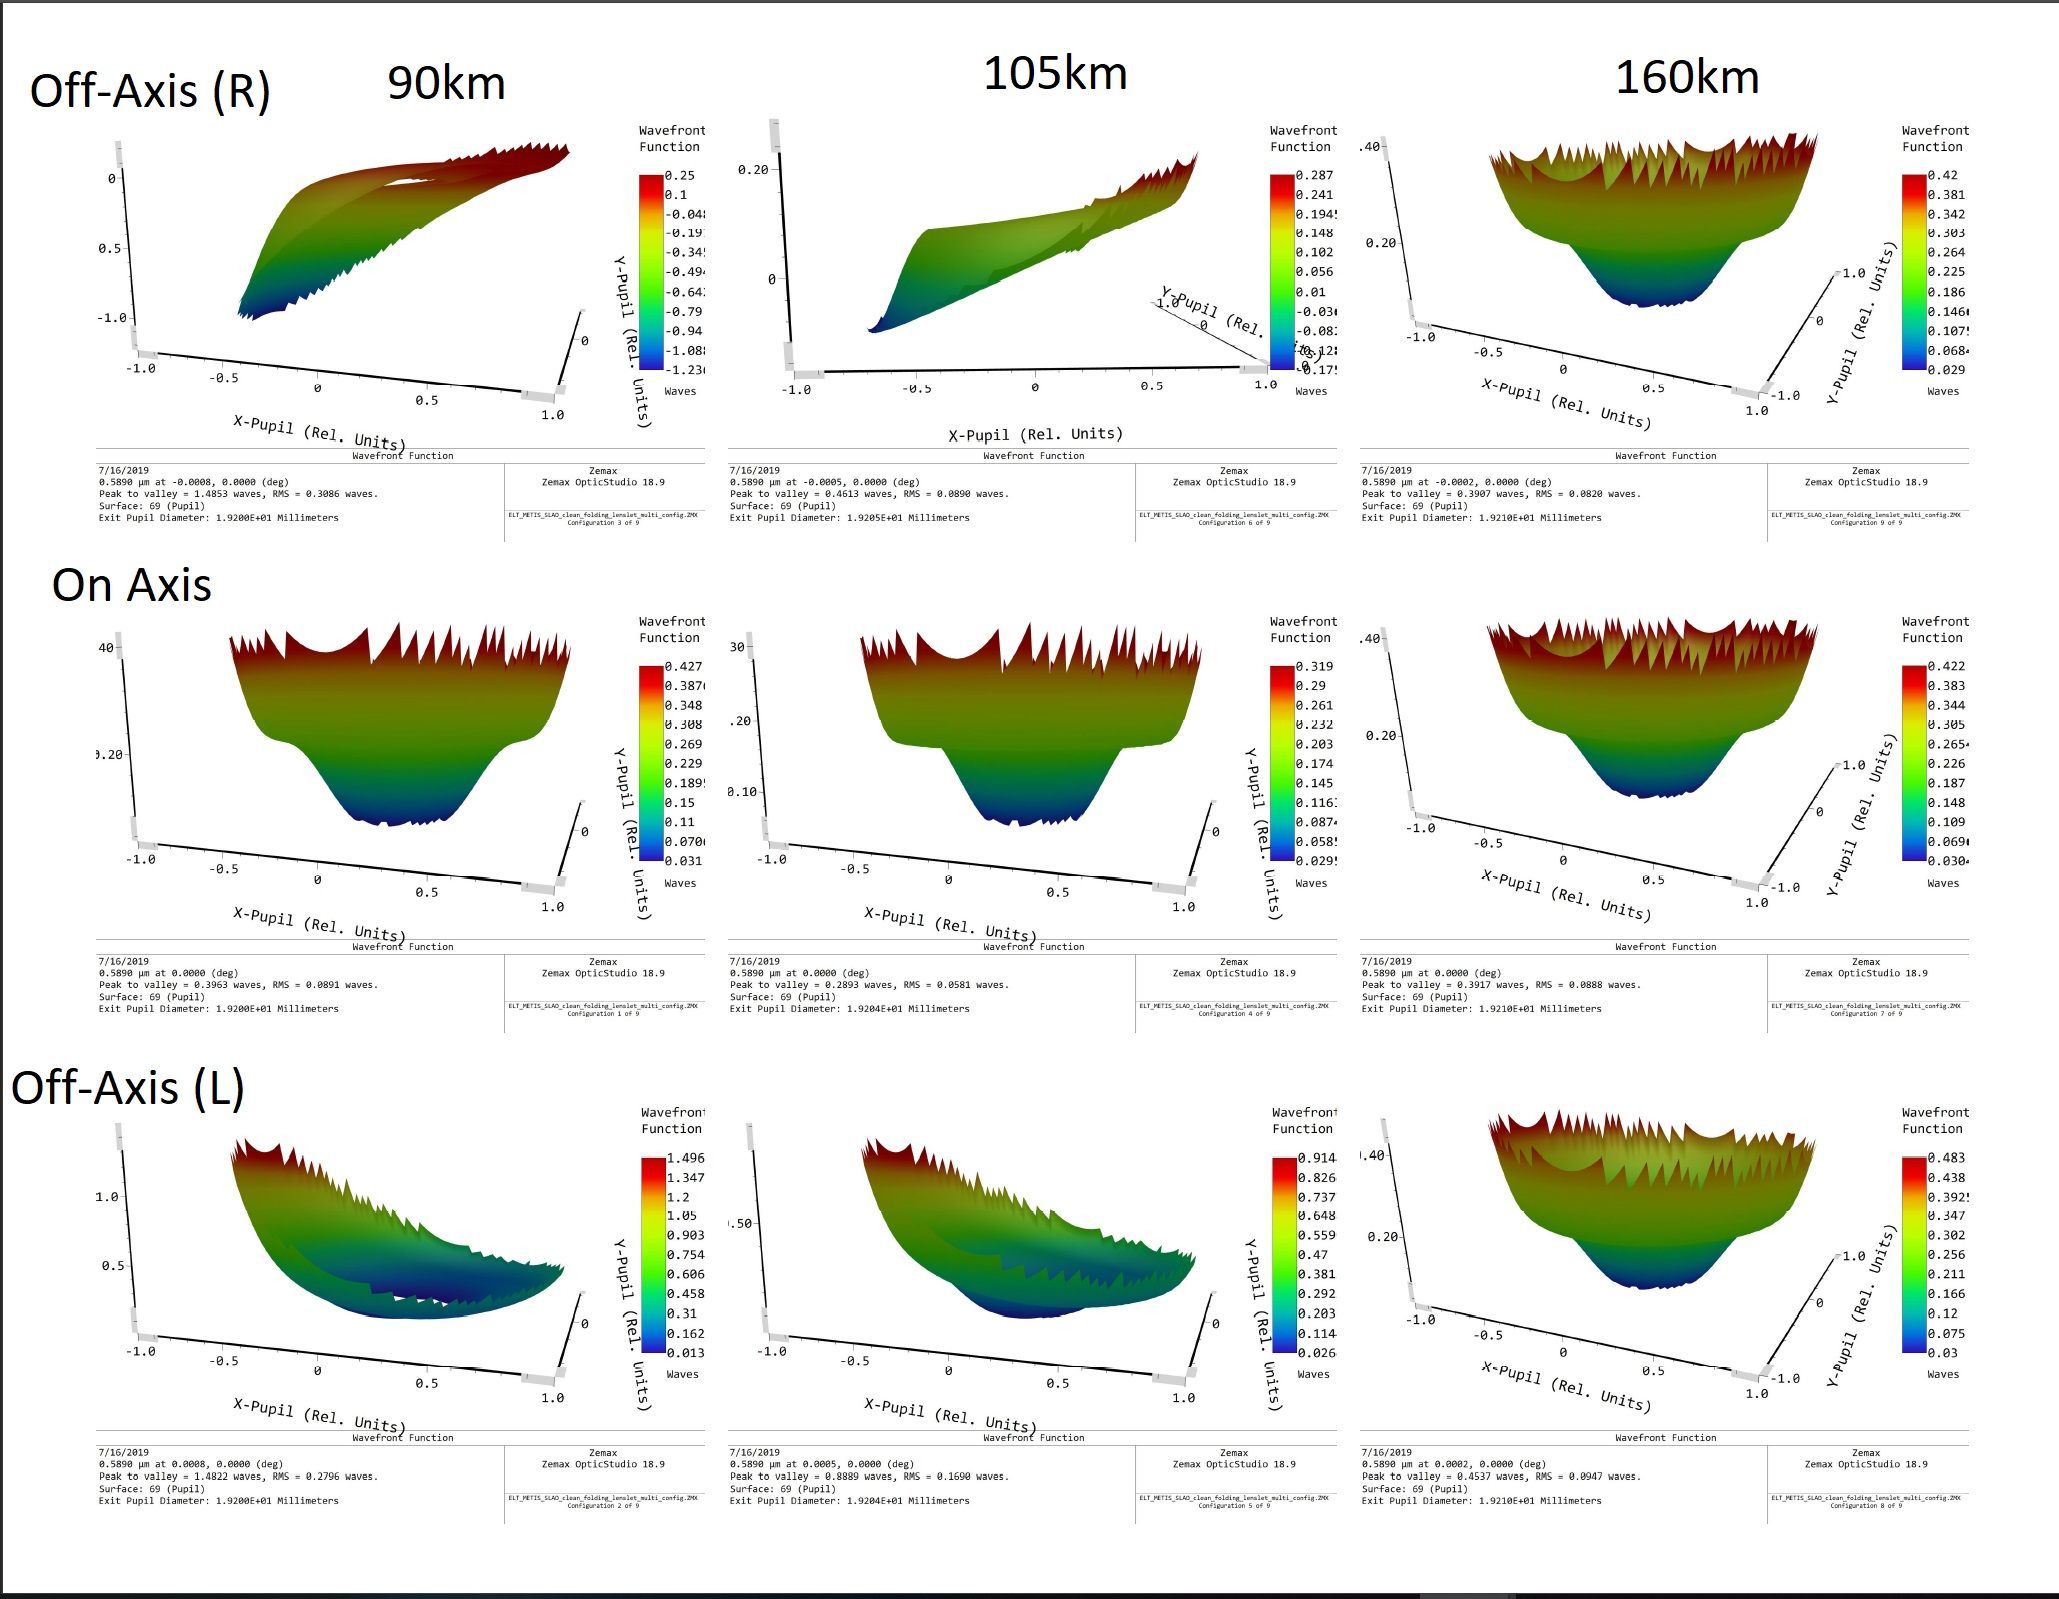
\includegraphics[width=14 cm]{Figures/wavefront_all.jpg}
\caption{All wavefront maps for on axis and off axis spots at different Zenith angles}
% \label{fig:metis_over}
\end{figure}
%% Appendix A

\chapter{Simulation Results} % Main appendix title

\label{AppendixB} % For referencing this appendix elsewhere, use \ref{AppendixA}

\begin{figure}[H]
    \centering
    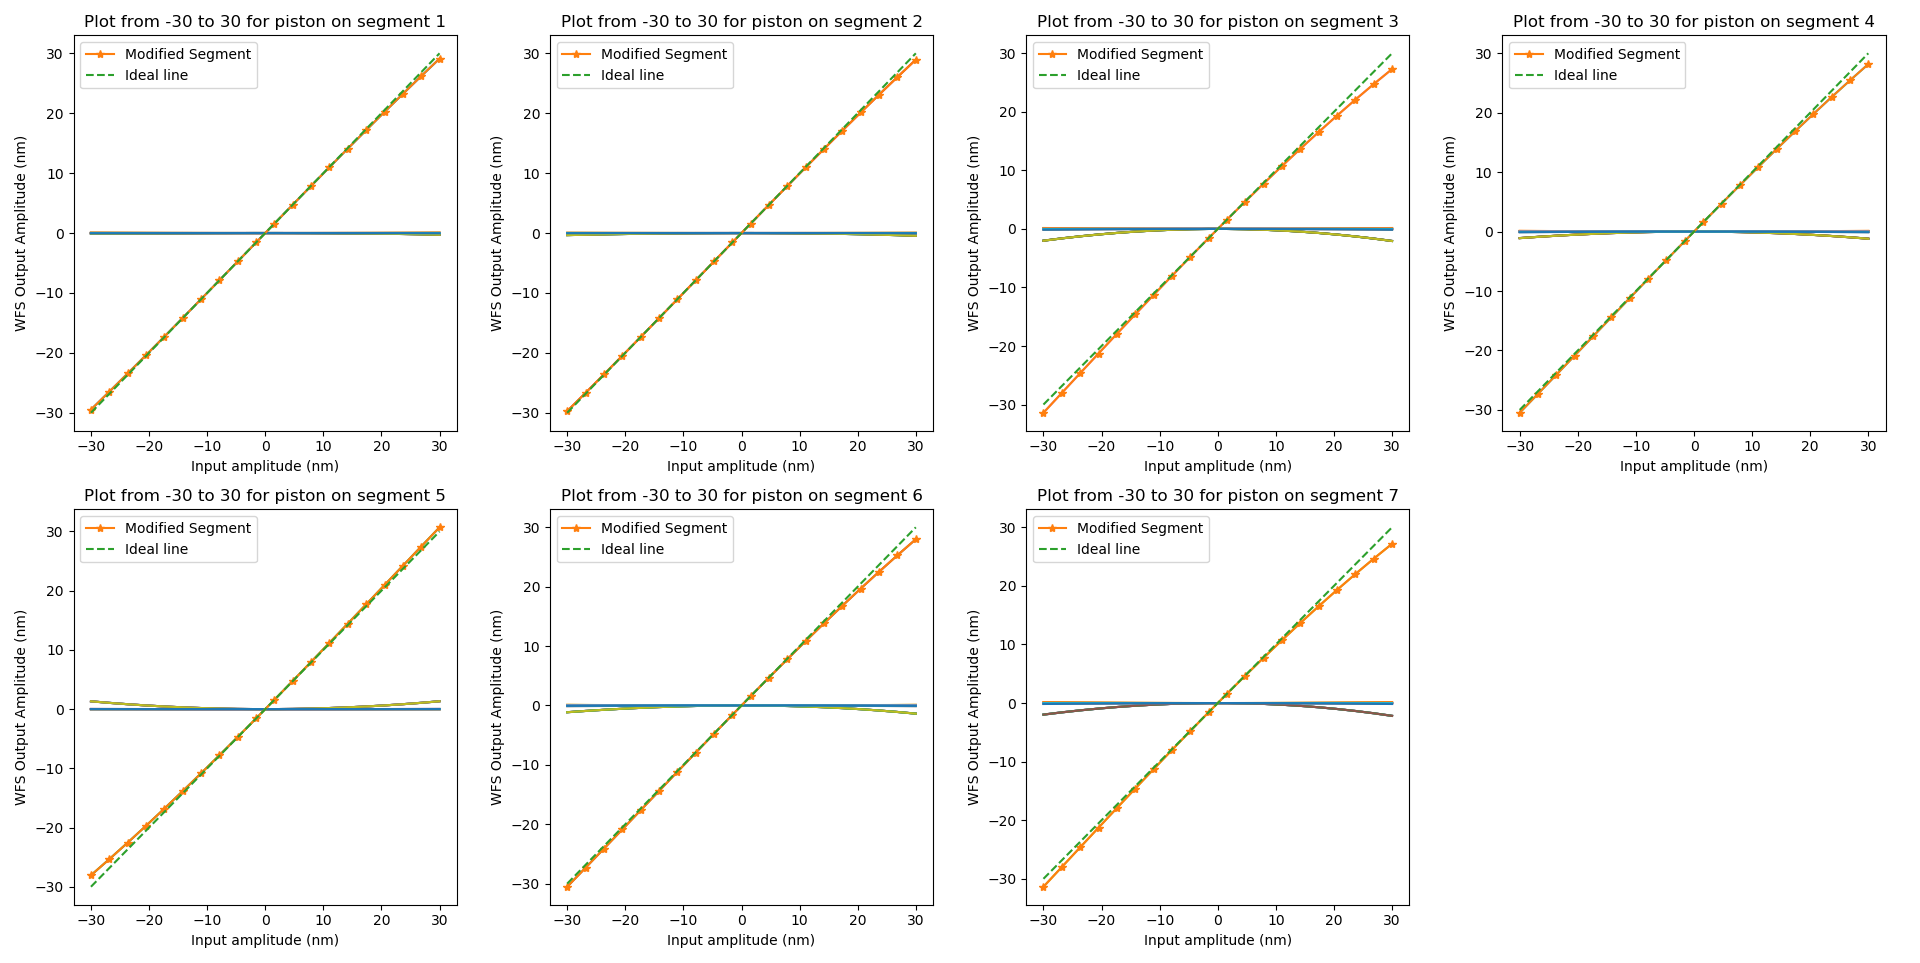
\includegraphics[width = 14cm]{Figures/Pist_response30.png}
    \caption{Piston correlation between -30 to 30 nm.}
    \label{fig:Pist30}
\end{figure}

\begin{figure}[H]
    \centering
    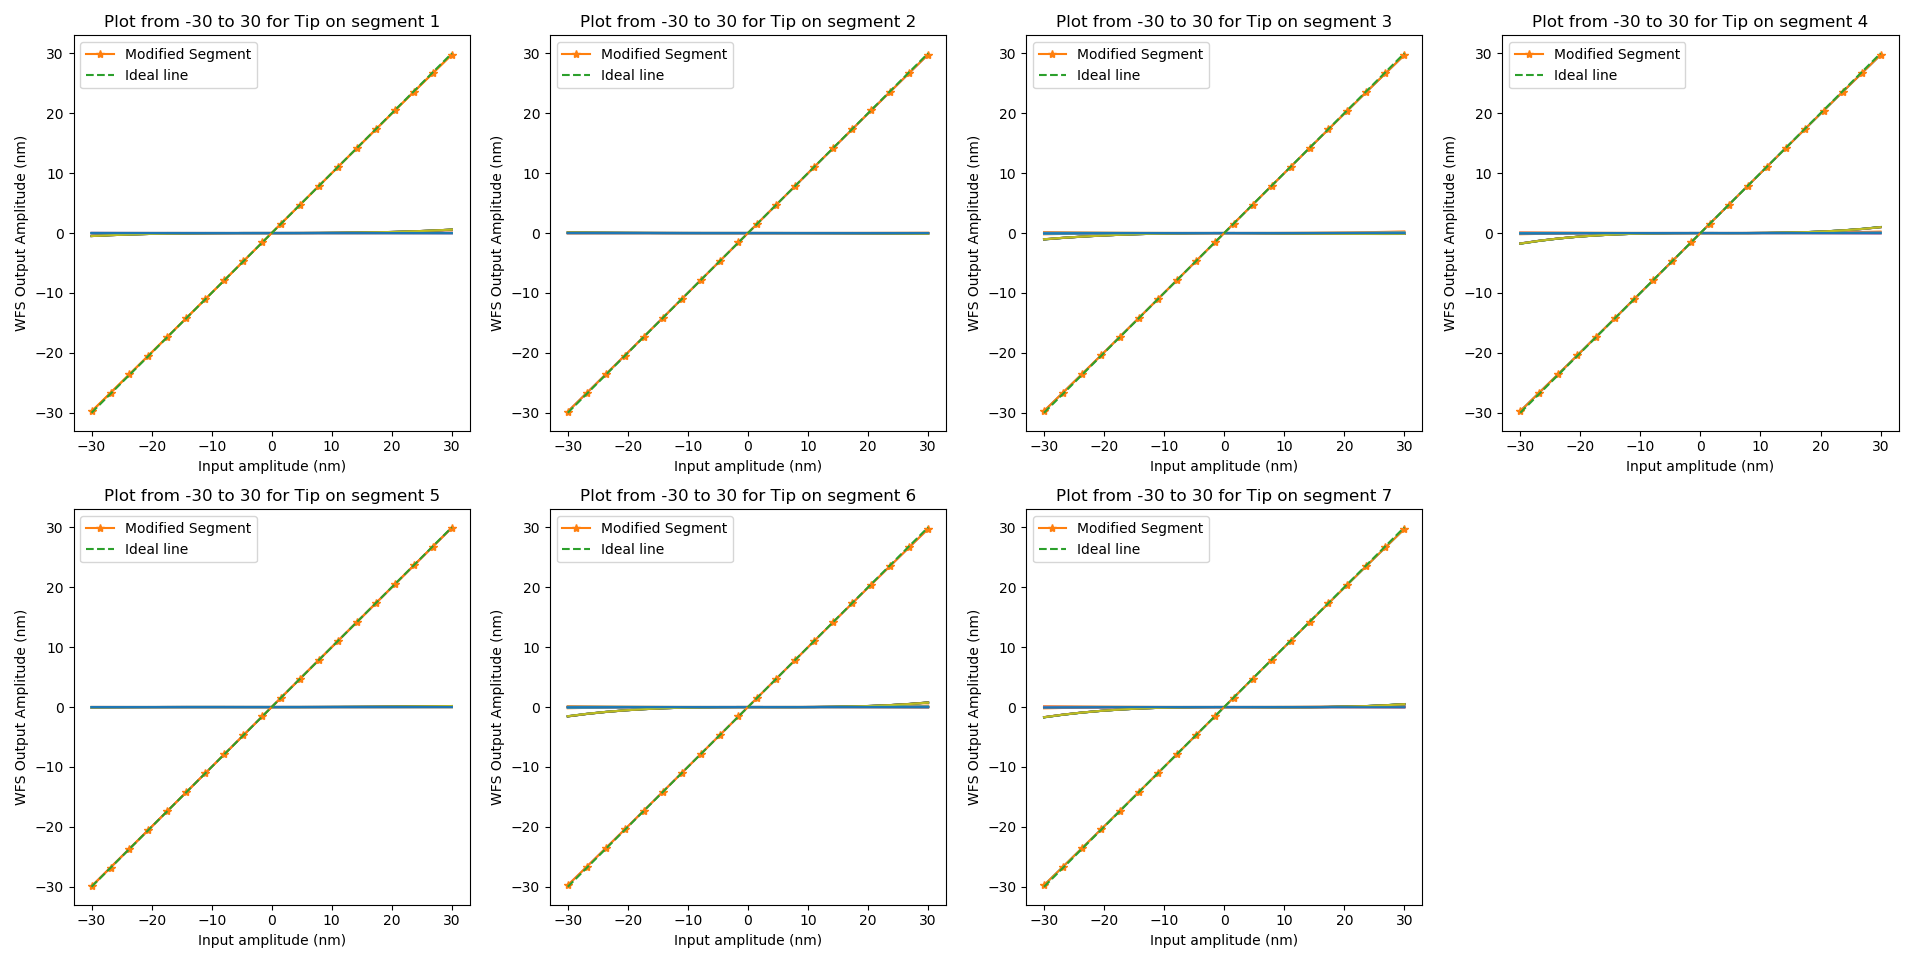
\includegraphics[width = 14cm]{Figures/Tip_response30.png}
    \caption{Tip correlation between -30 to 30 nm.}
    \label{fig:tip30}
\end{figure}

\begin{figure}[H]
    \centering
    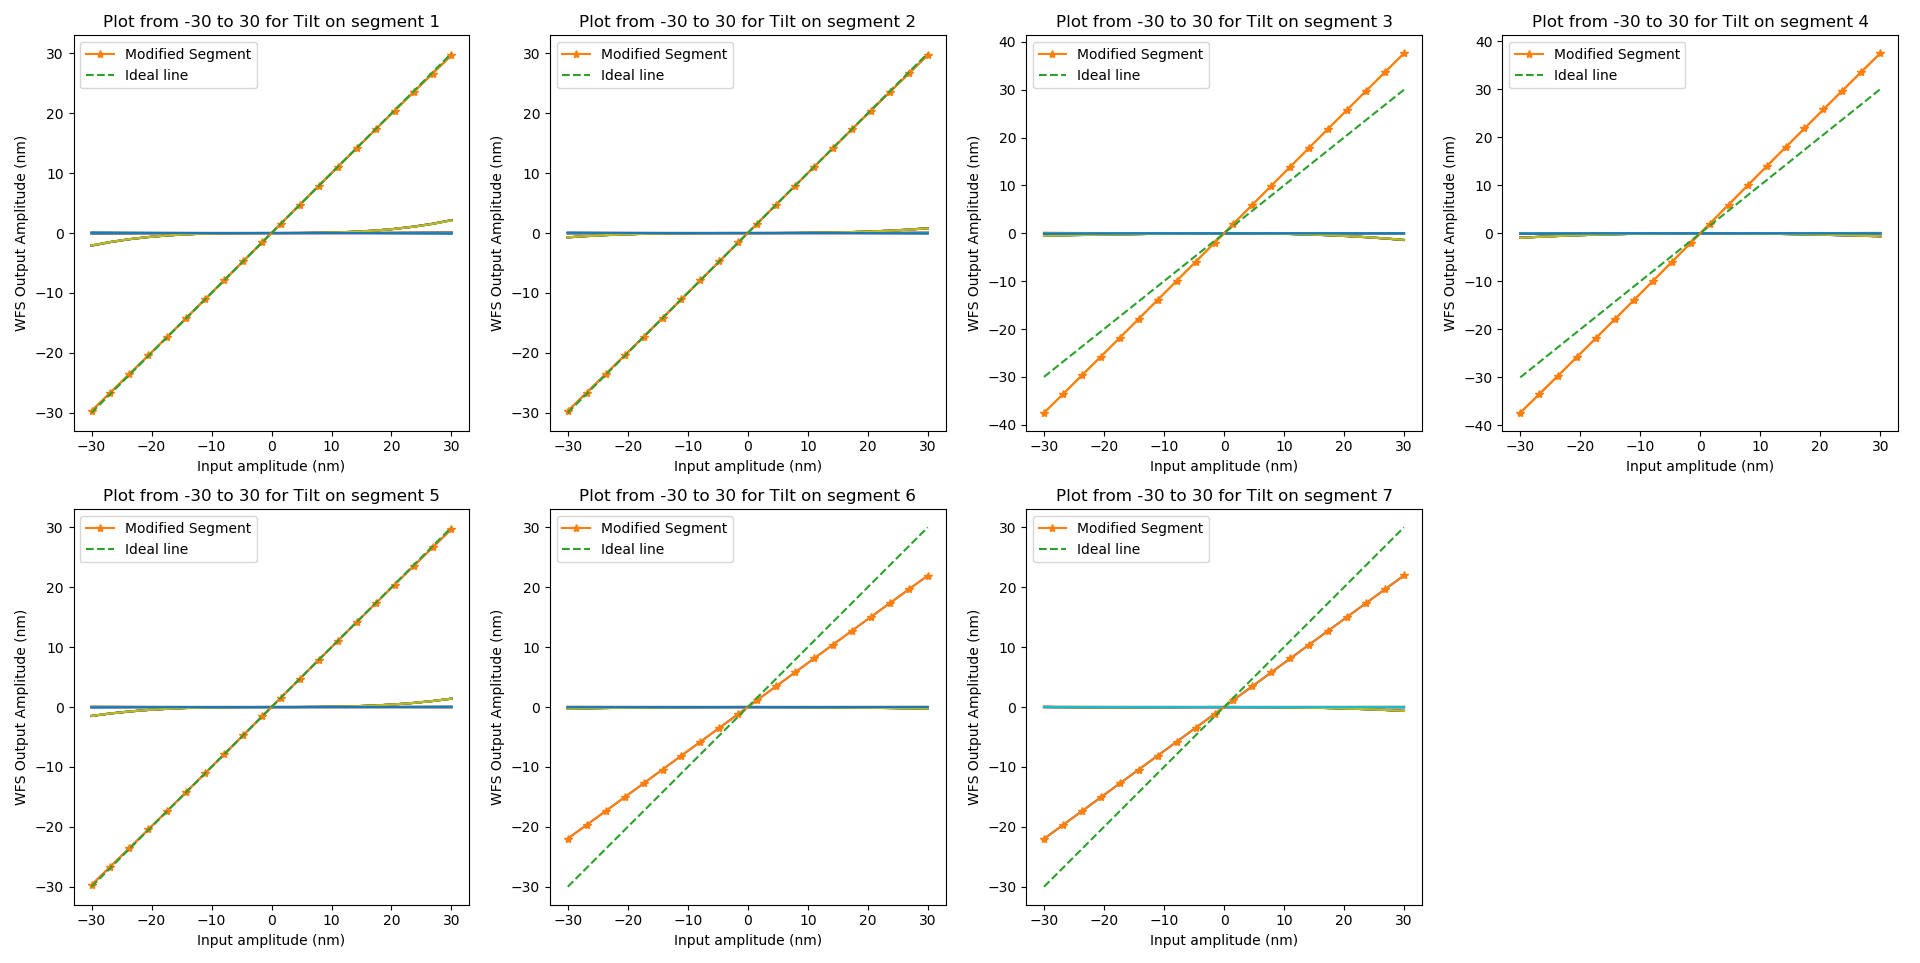
\includegraphics[width = 14cm]{Figures/Tilt_response30.png}
    \caption{Tilt correlation between -30 to 30 nm.}
    \label{fig:Tilt30_app}
\end{figure}
%\include{Appendices/AppendixC}

%----------------------------------------------------------------------------------------
%	BIBLIOGRAPHY
%----------------------------------------------------------------------------------------

\printbibliography
% \bibliography{example.bib}

%----------------------------------------------------------------------------------------

\end{document}  
